%%%%%%%%%%%%%%%%%%%%%%%%%%%%%%%%%%%%%%%%%
% Masters/Doctoral Thesis 
% LaTeX Template
% Version 2.5 (27/8/17)
%
% This template was downloaded from:
% http://www.LaTeXTemplates.com
%
% Version 2.x major modifications by:
% Vel (vel@latextemplates.com)
%
% This template is based on a template by:
% Steve Gunn (http://users.ecs.soton.ac.uk/srg/softwaretools/document/templates/)
% Sunil Patel (http://www.sunilpatel.co.uk/thesis-template/)
%
% Template license:
% CC BY-NC-SA 3.0 (http://creativecommons.org/licenses/by-nc-sa/3.0/)
%
%%%%%%%%%%%%%%%%%%%%%%%%%%%%%%%%%%%%%%%%%

%----------------------------------------------------------------------------------------
%	PACKAGES AND OTHER DOCUMENT CONFIGURATIONS
%----------------------------------------------------------------------------------------

\documentclass[
11pt, % The default document font size, options: 10pt, 11pt, 12pt
%oneside, % Two side (alternating margins) for binding by default, uncomment to switch to one side
english, % ngerman for German
singlespacing, % Single line spacing, alternatives: onehalfspacing or doublespacing
%draft, % Uncomment to enable draft mode (no pictures, no links, overfull hboxes indicated)
%nolistspacing, % If the document is onehalfspacing or doublespacing, uncomment this to set spacing in lists to single
%liststotoc, % Uncomment to add the list of figures/tables/etc to the table of contents
%toctotoc, % Uncomment to add the main table of contents to the table of contents
%parskip, % Uncomment to add space between paragraphs
%nohyperref, % Uncomment to not load the hyperref package
headsepline, % Uncomment to get a line under the header
%chapterinoneline, % Uncomment to place the chapter title next to the number on one line
consistentlayout, % Uncomment to change the layout of the declaration, abstract and acknowledgements pages to match the default layout
]{MastersDoctoralThesis} % The class file specifying the document structure

%\usepackage[utf8]{inputenc} % Required for inputting international characters
%\usepackage[T1]{fontenc} % Output font encoding for international characters

%\usepackage{mathpazo} % Use the Palatino font by default

\usepackage[backend=bibtex,style=numeric,natbib=true]{biblatex} % Use the bibtex backend with the authoryear citation style (which resembles APA)
\usepackage[autostyle=true]{csquotes} % Required to generate language-dependent quotes in the bibliography

\usepackage{soul} % Importing the package so as to be able to highlight specific lines

%\addbibresource{example.bib} % The filename of the bibliography
\addbibresource{Bibliography/EvoComp.bib} % The bibliography from all my previous research work



%----------------------------------------------------------------------------------------
%	MARGIN SETTINGS
%----------------------------------------------------------------------------------------

\geometry{
	paper=a4paper, % Change to letterpaper for US letter
	inner=2.5cm, % Inner margin
	outer=3.8cm, % Outer margin
	bindingoffset=.5cm, % Binding offset
	top=1.5cm, % Top margin
	bottom=1.5cm, % Bottom margin
	%showframe, % Uncomment to show how the type block is set on the page
}

%----------------------------------------------------------------------------------------
%	THESIS INFORMATION
%----------------------------------------------------------------------------------------

\thesistitle{Evolving Morphological Robustness for Collective Robotics} % Your thesis title, this is used in the title and abstract, print it elsewhere with \ttitle
\supervisor{Dr. Geoff \textsc{Nitschke}} % Your supervisor's name, this is used in the title page, print it elsewhere with \supname
\examiner{} % Your examiner's name, this is not currently used anywhere in the template, print it elsewhere with \examname
\degree{Master of Science} % Your degree name, this is used in the title page and abstract, print it elsewhere with \degreename
\author{A. Ruben \textsc{Putter}} % Your name, this is used in the title page and abstract, print it elsewhere with \authorname
\addresses{} % Your address, this is not currently used anywhere in the template, print it elsewhere with \addressname

\subject{Evolutionary Copmuting} % Your subject area, this is not currently used anywhere in the template, print it elsewhere with \subjectname
\keywords{} % Keywords for your thesis, this is not currently used anywhere in the template, print it elsewhere with \keywordnames
\university{\href{http://www.uct.ac.za}{University of Cape Town}} % Your university's name and URL, this is used in the title page and abstract, print it elsewhere with \univname
\department{\href{http://www.cs.uct.ac.za}{Department of Computer Science}} % Your department's name and URL, this is used in the title page and abstract, print it elsewhere with \deptname
\group{\href{http://researchgroup.university.com}{Research Group Name}} % Your research group's name and URL, this is used in the title page, print it elsewhere with \groupname
\faculty{\href{http://faculty.university.com}{Faculty of Science}} % Your faculty's name and URL, this is used in the title page and abstract, print it elsewhere with \facname

\AtBeginDocument{
\hypersetup{pdftitle=\ttitle} % Set the PDF's title to your title
\hypersetup{pdfauthor=\authorname} % Set the PDF's author to your name
\hypersetup{pdfkeywords=\keywordnames} % Set the PDF's keywords to your keywords
}

\begin{document}

\frontmatter % Use roman page numbering style (i, ii, iii, iv...) for the pre-content pages

\pagestyle{plain} % Default to the plain heading style until the thesis style is called for the body content

%----------------------------------------------------------------------------------------
%	TITLE PAGE
%----------------------------------------------------------------------------------------

\begin{titlepage}
\begin{center}

\vspace*{.06\textheight}
{\scshape\LARGE \univname\par}\vspace{1.5cm} % University name
\textsc{\Large Masters Thesis}\\[0.5cm] % Thesis type

\HRule \\[0.4cm] % Horizontal line
{\huge \bfseries \ttitle\par}\vspace{0.4cm} % Thesis title
\HRule \\[1.5cm] % Horizontal line
 
\begin{minipage}[t]{0.4\textwidth}
\begin{flushleft} \large
\emph{Author:}\\
\href{http://www.johnsmith.com}{\authorname} % Author name - remove the \href bracket to remove the link
\end{flushleft}
\end{minipage}
\begin{minipage}[t]{0.4\textwidth}
\begin{flushright} \large
\emph{Supervisor:} \\
\href{http://www.jamessmith.com}{\supname} % Supervisor name - remove the \href bracket to remove the link  
\end{flushright}
\end{minipage}\\[3cm]
 
\vfill

\large \textit{A thesis submitted in fulfillment of the requirements\\ for the degree of \degreename}\\[0.3cm] % University requirement text
\textit{in the}\\[0.4cm]
\groupname\\\deptname\\[2cm] % Research group name and department name
 
\vfill

{\large \today}\\[4cm] % Date
%\includegraphics{Logo} % University/department logo - uncomment to place it
 
\vfill
\end{center}
\end{titlepage}

%----------------------------------------------------------------------------------------
%	DECLARATION PAGE
%----------------------------------------------------------------------------------------

\begin{declaration}
\addchaptertocentry{\authorshipname} % Add the declaration to the table of contents
\noindent I, \authorname, declare that this thesis titled, \enquote{\ttitle} and the work presented in it are my own. I confirm that:

\begin{itemize} 
\item This work was done wholly or mainly while in candidature for a research degree at this University.
\item Where any part of this thesis has previously been submitted for a degree or any other qualification at this University or any other institution, this has been clearly stated.
\item Where I have consulted the published work of others, this is always clearly attributed.
\item Where I have quoted from the work of others, the source is always given. With the exception of such quotations, this thesis is entirely my own work.
\item I have acknowledged all main sources of help.
\item Where the thesis is based on work done by myself jointly with others, I have made clear exactly what was done by others and what I have contributed myself.\\
\end{itemize}
 
\noindent Signed:\\
\rule[0.5em]{25em}{0.5pt} % This prints a line for the signature
 
\noindent Date:\\
\rule[0.5em]{25em}{0.5pt} % This prints a line to write the date
\end{declaration}

\clearpage

%----------------------------------------------------------------------------------------
%	QUOTATION PAGE
%----------------------------------------------------------------------------------------

\vspace*{0.2\textheight}

\noindent\enquote{\itshape Thanks to my solid academic training, today I can write hundreds of words on virtually any topic without possessing a shred of information, which is how I got a good job in journalism.}\bigbreak

\hfill Dave Barry

%----------------------------------------------------------------------------------------
%	ABSTRACT PAGE
%----------------------------------------------------------------------------------------

\begin{abstract}
\addchaptertocentry{\abstractname} % Add the abstract to the table of contents
The Thesis Abstract is written here (and usually kept to just this page). The page is kept centered vertically so can expand into the blank space above the title too\ldots
\end{abstract}

%----------------------------------------------------------------------------------------
%	ACKNOWLEDGEMENTS
%----------------------------------------------------------------------------------------

\begin{acknowledgements}
\addchaptertocentry{\acknowledgementname} % Add the acknowledgements to the table of contents
The acknowledgments and the people to thank go here, don't forget to include your project advisor\ldots
\end{acknowledgements}

%----------------------------------------------------------------------------------------
%	LIST OF CONTENTS/FIGURES/TABLES PAGES
%----------------------------------------------------------------------------------------

\tableofcontents % Prints the main table of contents

\listoffigures % Prints the list of figures

\listoftables % Prints the list of tables

%----------------------------------------------------------------------------------------
%	ABBREVIATIONS
%----------------------------------------------------------------------------------------

\begin{abbreviations}{ll} % Include a list of abbreviations (a table of two columns)

\textbf{LAH} & \textbf{L}ist \textbf{A}bbreviations \textbf{H}ere\\
\textbf{WSF} & \textbf{W}hat (it) \textbf{S}tands \textbf{F}or\\

\end{abbreviations}

%----------------------------------------------------------------------------------------
%	PHYSICAL CONSTANTS/OTHER DEFINITIONS
%----------------------------------------------------------------------------------------

\begin{constants}{lr@{${}={}$}l} % The list of physical constants is a three column table

% The \SI{}{} command is provided by the siunitx package, see its documentation for instructions on how to use it

Speed of Light & $c_{0}$ & \SI{2.99792458e8}{\meter\per\second} (exact)\\
%Constant Name & $Symbol$ & $Constant Value$ with units\\

\end{constants}

%----------------------------------------------------------------------------------------
%	SYMBOLS
%----------------------------------------------------------------------------------------

\begin{symbols}{lll} % Include a list of Symbols (a three column table)

$a$ & distance & \si{\meter} \\
$P$ & power & \si{\watt} (\si{\joule\per\second}) \\
%Symbol & Name & Unit \\

\addlinespace % Gap to separate the Roman symbols from the Greek

$\omega$ & angular frequency & \si{\radian} \\

\end{symbols}

%----------------------------------------------------------------------------------------
%	DEDICATION
%----------------------------------------------------------------------------------------

\dedicatory{For/Dedicated to/To my\ldots} 

%----------------------------------------------------------------------------------------
%	THESIS CONTENT - CHAPTERS
%----------------------------------------------------------------------------------------

\mainmatter % Begin numeric (1,2,3...) page numbering

\pagestyle{thesis} % Return the page headers back to the "thesis" style

% Include the chapters of the thesis as separate files from the Chapters folder
% Uncomment the lines as you write the chapters

% Chapter 1

\chapter{Introduction} % Main chapter title

\label{Chapter1} % For referencing the chapter elsewhere, use \ref{Chapter1}

%----------------------------------------------------------------------------------------

% Define some commands to keep the formatting separated from the content
\newcommand{\keyword}[1]{\textbf{#1}}
\newcommand{\tabhead}[1]{\textbf{#1}}
\newcommand{\code}[1]{\texttt{#1}}
\newcommand{\file}[1]{\texttt{\bfseries#1}}
\newcommand{\option}[1]{\texttt{\itshape#1}}

%----------------------------------------------------------------------------------------

\section{Introduction}



% 1 = \cite{Beni2004}
% 2 = \cite{BongardZykovLipson2006}
% 3 = \cite{BrooksFlynn1989}
% 5 = \cite{CullyCluneTaraporeMouret2015}
% 8 = \cite{DoncieuxBredecheMouretEiben2015}
% 10 = \cite{fenton2001fault}
% 21 = \cite{verma2004real}

% "Autonomous robots are increasingly being applied to remote and hazardous environments [3,1], environments damage to sensory actuator systems cannot be easily repaired if damaged. An unsolved problem in the controller design for such autonomous robots is having controllers continue to effectively function given unexpected changes such as damage to robot morphology."

% "Currently, robotic systems recover from damage via self diagnosis and selection from pre-designed contingency plans in order to continue functioning [10,21,2]. Though robots using such self-diagnosis and recovery are problematic systems as they are expensive, requiring sophisticated monitoring sensors, and difficult to design as a priori knowledge of all necessary contingency plans is assumed [5]""

% "Addressing this, recent work in Evolutionary Robotics [8] elucidated the efficacy of population based stochastic trial and error methods for online damage recovery in autonomous robots operating in physical environments [5]. This was demonstrated as being akin to self-adaptation and injury recovery of animals observed in nature.""

% "This study further contributes to this research area, focussing on evolutionary controller design [11] within the broader context of collective [15] and swarm [1] robotics. That is, evolutionary controller design for robot groups that must continue to accomplish tasks given that damage is sustained to the morphologies of some or all of the robots in the group. ""

% ====================================================
The design and development of automated problem solvers and autonomous robots has long been a central theme of research in the crossover between artificial intelligence and robotics \cite{RefWorks:33}. However, given the levels of complexity and non-linearity of real-world problems, traditional methods of controller design have become impractical since they rely mostly on linear mathematical models \cite{RefWorks:32}. An additional consideration is that at a certain point, designing the problem solver becomes more difficult than solving the problem, especially when there is not a distinct and well-defined set of steps to follow in order to obtain the solution.

One such complex task, and the one being focussed on as the subject of this thesis, is that of achieving automated collective behaviour in which a team of autonomous agents must cooperate amongst themselves in order to accomplish a task. More specifically, this thesis will focus on collective robotics with a case study on the collective construction task

While it may be possible to to solve many complex tasks using a single sophisticated robot, there are several advantages to using collective robotics instead. Some of these advantages include being able to use much simpler designed robots in the team instead of one very expensive robot as well as having increased fault tolerance since there is no longer a single point of failure \cite{chaimowicz2001architecture}. The downside to a multi-agent team, however, is the infeasibility of designing the intricate dynamics inherent in producing self-organised behaviour between individuals by hand \cite{RefWorks:11}.

The collective construction task requires that a team of agents cooperate by coordinating their behaviours in order to assemble various structures within their environment \cite{NitschkeSaEC2012}. A group of autonomous agents (robots) are deployed into an unknown environment which they must explore in order to find resources and figure out how to assemble these resources in such a way as to create some structure, which can be completely predefined, or just according to some predefined structural criteria \cite{NitschkeSaEC2012}.

The ability to automate construction tasks through creating controllers for collective robotics presents several considerable benefits. Automation like this could be used to assist in projects such as producing low-cost housing in locations where resources are scarce, reducing high accident rates due to human error which is unfortunately unavoidable in traditional construction methods \cite{ShenKhoshnevis2003}. An additional possible application in the near future is to send multi-robot construction teams to extraterrestrial planets in order to build habitable structures in anticipation of humans arriving. These robot teams would also be useful in underwater construction which is extremely difficult and is one of the most dangerous jobs \cite{RefWorks:30}.

In an attempt to try and find a solution around the complexity of automating the design of these controllers, researchers turned to biological and natural processes for inspiration.

The problem solving power of evolution is abundantly clear in nature with the diverse range of organisms that exist (or ever have existed) on Earth, each specially designed for optimal survival in its own niche environment \cite{RefWorks:33}, making it unsurprising that computer scientists have resorted to researching natural processes for inspiration. 

One such approach that draws inspiration from Darwinian evolution is Evolutionary Algorithms which relates the fundamental metaphor of the evolutionary process to a simple style of problem solving, which is that of trial-and-error (also referred to as generate-and-test) \cite{RefWorks:33}.

\hl{"For the time being, let us consider natural evolution simply as follows. A given environment is filled with a population of individuals that strive for survival and reproduction. The fitness of these individuals - determined by the environment - relates to how well they succeed in achieving their goals, i.e., it represents their chances of survival and multiplying."} \cite{EibenSmith2003}

These algorithms work by performing actions that are analagous to the process of Natural Selection (reproduction to produce subsequent generations, gene cross-over and mutation)

\hl{"Natural selection favours those individuals that compete for the given resources most effectively, in other words, those that are adapted or fit to the environmental conditions best. This phenomenon is also known as Survival Of The Fittest."} \cite{EibenSmith2003}




\hl{"Competition-based selection is the one of the two cornerstones of evolutionary progress. The other primary force identified by Darwin results from phenotypic variations among members of the population. Phenotypic traits aare those behavioural and physical features of an individual that directly affect its response to the environment (including other individuals), thus determining its fitness."} \cite{EibenSmith2003}


%%	OVERVIEW OF THE TECHNOLOGY -- CAN POSSIBLY PUT THIS IN A SECTION IN CHAPTER 2?	
Structure of the research field itself: \cite{EibenSmith2003}
Based on a technology called "Evolutionary Computing"
	-> the algorithms used by this technology are called "Evolutionary Algorithms"
	-> considers Evolutionary Programming, Evolution Strategies, Genetic Algorithms, Genetic Programming as subareas of EC belonging to the corresponding algorithm variants
%%%%%%%%%%%%%%%%%%%%%%%%%%%%%%%%%%%%%%%%%%%%%%%%%%%%%%%%%%%%%%%

One such example of an Evolutionary Computing approach, and the method being investigated in this thesis, is called Neuroevolution and it works by combining Genetic Algorithms/Genetic Programming in order to train ANN's.


\hl{"Accidents happen in nature from simple incidents like bumping into obstacles, to erroneously arriving at the wrong location, to mating with an unintended partner. Whether accidents are problematic for an animal depends on their context, frequency, and severity."} \cite{ferreira2018accidental}.

\hl{"In this paper, we investigate the question of how accidents affect the task performance of agents in an agent-based simulation modelf for a wide class of tasks call 'Multi-Agent Territory Exploration' (MATE). In MATE tasks, agents have to visit particular locations of varying quality in partially observbable environments within a fixed time window. As such, agents have to balance the quality of the location with how much energy they are willing to expend reaching it. Arriving at the wrong location by acccident, typically reduces task performance."} \cite{ferreira2018accidental}.

\hl{"We model agents based on two location selection strategies that are hypothesized to be widely used in nature: best-of-n and min-threshold. Our results show that the two strategies lead to different accident rates and thus overall different levels of performance based on the degree of competition among agents, as well as the quality, density, visibility, and distribution of target locations in the environment. We also show that in some cases individuual accidents can  be advantageous for noth the individual and the whole group"} \cite{ferreira2018accidental}



%% The below can be used somewhere like Future Work or Considerations in the Experiments:
\hl{"Evolutionary processes can be simulated in a computer, where millions of generations can be executed in a matter of hours or days and repeated under various circumstances. These possibilities go far beyond studies based on excavations and fossils, or those possible 'in vivo'. Naturally, the interpretation of such simulation experiments must be done very carefully. First, because we do not know whether the computer models represent the biological reality with sufficient fidelity. Second, it is unclear whether conclusions drawn in a digital medium, 'in silico', can be transferred to the carbon-based biological medium. These caveats and the lack of mutual awareness between biologists and computer scientists are probably the reason why there are few computer experimental studies about fundamental issues of biological evolution"} \cite{EibenSmith2003}.


====== Motivation for investigating Novelty Search can be explained as being analagous to accidental encounters being beneficial or adaptive =======

\hl{"Take, for example, the common instance3 of a MATE task where agents (eg. females) attempt to find (stationary) mates located in the environment using different mate selection strategies based on males's mating calls or displays of prowess, which are indicative of the quality of the mate and thus a crucial determinant of the quality of the offspring. Since females typically only have partial knowledge of the location of possible partners, as some males mayt not advertise their location through calls, they may end up mating with non-optimal partners by accident (eg. bumping into a potential mate causes females to simply mate with the male in some species such as tree frogs). For low quality males who might not win in a 'shouting' competition with high quality males, it might thus be beneficial to remain silent and try to intercept females instead of calling, a strategy often referred to as 'satellite' strategy; for if they decide to call, females might actively avoid them."} \cite{ferreira2018accidental}
-- The above has original references as well -> check page 2/20 LHS for full references

Based on the above described patterns in natural interactions between individuals, this study also investigates the efficacy of Novelty Search as a fitness function in the Evolutionary Algorithm.



===============================================================
EDIT 1:
-----------------------
ADD SOME REAL WORLD EXAMPLES AND DESCRIPTIONS OF NE 
"NE is the main method for controller adaptation in evolutionary robotics (the overall topic that this thesis fits into) - and within this field - NE applied to collective robotics has achieved success (evolved effective group behaviours) to solve various collective behaviour tasks - then give several example tasks that evolutionary collective robotics systems have solved - with references"
==================================================================

Within the purview of collective robotics, NE is the main method used for controller evolution

Neuroevolution (NE) is a method of artificially evolving Artificial Neural Networks (ANN's) by implementing Evolutionary Algorithms to perform tasks such as evolving the network connection weights as well as the network topology \cite{Stanley2004, XinYao1999}.

Given that there are several learning tasks in the real world, such as game playing, vehicle control, and robotics, that are not well-suited to supervised learning methods, Neuroevolution aims to find an ANN that optimizes behaviour given only sparse information regarding how WELL the agents are performing, and without any input on WHAT they should be doing \cite{Miikkulainen2010}. 
In the above outlined scenarios, the optimal action at each timestep is not always known and can only be determined after performing several actions to get information about the outcome of those actions and whether or not it was beneficial given the defined parameters \cite{Miikkulainen2010}.
This makes Neuroevolution a suitable approach for this dissertation/research as it falls within the specialised problem-space.

\hl{"Neuroevolution is a combination of neural networks and Genetic Algorithms where neural networks are the phenotype being evaluated"} \cite{Stanley2004}.

\hl{"The genotype is a compact representation that can be translated into an artificial neural network. NE searches for neural networks that optimize some performance measure. NE can search for virtually any kind of neural network whether it be simple, feed-forward, recurrent, or even adaptive networks"} \cite{Stanley2004}.

When compared to various other neural network learning methods, NE can be observed to be highly general. This allows for learning to be performed without explicit targets, with non-differentiable activation functions, as well as recurrent networks \cite{Miikkulainen2010}.

\hl{"As long as the performance of the networks can be evaluated over time, and the behaviour of the network can be modified through evolution, it can be applied to a wide range of network architectures, including those with nondifferentiable activation functions and recurrent and higher-order connections"} \cite{Miikkulainen2010}.

\hl{"Neuroevolution allows combining evolution over a population of solutions with lifetime learning in individual solutions: the evolved networks can each learn further through eg. Backpropagation or Hebbian learning."} \cite{Miikkulainen2010}.

It makes use of Evolutionary Algorithms in order to abstract the key aspects of the evolutionary process into a generational loop that will search for an optimal solution out of a population of candidates by evaluating each one in order to determine which is the fittest and thus the characteristics that persist to the next generation. Resulting in a stochastic search for the most optimal solution of the problem space.

The different types of NE methods can be roughly/generally broken down into two different categories, with respect to the encoding method used to map an individual agent's genotype to its phenotype (from PTTAND010_Literature_Review.pdf)



\hl{Direct Encoding: NEAT}

In direct encoding methods, each element in the genotype explicitly encodes an independent aspect of the phenotype, such that there is a one-to-one mapping between the genotype and the phenotype \cite{clune2011performance, stanley2009hypercube}.

In this encoding scheme, all the parameters of an ANN's architecture are explicitly encoded on the chromosome as binary strings \cite{Gomez2003}. Each gene in the chromosome directly relates to a specific part of the network, allowing for a direct one-to-one mapping from the genotype to the phenotype \cite{StanleyMiikkulainen2002}.

The direct encoding scheme is relatively straight-forward to implement and it allows for a single connection to be easily added or removed from an ANN, making it suitable for precise fine-tuning of an architecture \cite{StanleyMiikkulainen2002}.
It may also accommodate for optimization and generation of unexplored architectures \cite{miller1989designing}.

On the other hand, a major disadvantage of direct encoding schemes is that it does not scale well \cite{XinYao1999}.  The reason for this is that the components of the network are mapped directly onto the chromosome, meaning there is no compression of information and would become computationally expensive as the size of the network grows.

An example of one such algorithm that makes use of a direct encoding method, is the Neuroevolution of Augmenting Topologies algorithm, also referred to as NEAT \cite{Gomez2003}.

NEAT is initialised with a small population of simple networks which are then gradually made more complex by either adding, removing, or mutating network connections \cite{RefWorks:11, Gomez2003}.


\hl{Indirect Encoding: HyperNEAT}

This encoding scheme functions at a higher level of abstraction than direct encoding  \cite{Gomez2003}.

An example implementation method of this encoding scheme includes using parametric functions to represent genes in a chromosome and using predetermined developmental rules to construct architectures \cite{koutnik2010evolving}.

In indirect encoding (also referred to as generative or developmental encoding) methods, each element in the genotype is implicitly described by computable function allowing for a much more compact representation of the genotype \cite{clune2011performance, stanley2009hypercube}. It also allows for genetic information to be re-used.

In other words, this algorithm transforms (decodes) the genotype to the phenotype by using any computable function \cite{koutnik2010evolving}.






It has been shown that NE can successfully be applied to complex control tasks that require collective behaviour. These control tasks have no obvious mappings between the input from sensory configurations and motor outputs \cite{NitschkeSaEC2012}.


%%%%%%%%%%%%%%%%%%%% EXAMPLE APPLICATIONS REAL WORLD %%%%%%%%%%%%%%%%

"Disaster rescue is one of the most serious social issues which involve a very large number of heterogeneous agents in the hostile environment. "\cite{KitanoTadokoro1999}


One of the biggest issues to overcome in order to make these agents as robust as possible (and more suited to their inherently dangerous environments) is determining some way for the robots to be able to continue performing their required tasks despite any physical damage to their physical morphology that they may sustain. More specifically, with regards to their sensory input devices, which are integral to the functioning of any agent.

In fact, an open problem in \textit{collective} \cite{KubeZhang1994B} and \textit{swarm robotics} \cite{Beni2004}
is ascertaining appropriate sensory-motor configurations (morphologies) for robot teams that must work collectively given automatically generated controllers \cite{FloreanoDurrMattiussi2008}.

Current robotic systems make use self-diagnosis and selection from pre-designed contingency plans in order to be able to recover from damage and continue its normal functioning \cite{fenton2001fault, verma2004real, BongardZykovLipson2006}. However, robots that implemented this approach of self-diagnosis and recovery proved to be somewhat problematic in that these systems are relatively expensive and are difficult to design since it requires full \textit{a priori} knowledge of the system in order to design the contingency plans \cite{CullyCluneTaraporeMouret2015}.












%%%%%%%%%%%%%%%%%%%%%%%%%%%%%%%%%%%%%%%%%%%%%%%%%%%%%%%%%%%%%%%%%%%%%
%% 					From the AAMAS Extended Abstract 		       %%
%%		Move this part below to the Research Objectives section    %%
%%%%%%%%%%%%%%%%%%%%%%%%%%%%%%%%%%%%%%%%%%%%%%%%%%%%%%%%%%%%%%%%%%%%%

Addressing this, recent work in \textit{Evolutionary Robotics} elucidated the efficacy of population based stochastic trial-and-error methods for online damage recovery in autonomous robots operating in physical environments \cite{CullyCluneTaraporeMouret2015}.
This was demonstrated as being akin to self-adaptation and injury recovery of animals observed in nature.

This study further contributes to this research area, focussing on \textit{evolutionary controller design} \cite{FloreanoDurrMattiussi2008} within the broader context of \textit{collective} \cite{KubeZhang1994B} and \textit{swarm} \cite{Beni2004} robotics.
That is, evolutionary controller design for robot groups that must continue to accomplish tasks given that damage is sustained to the morphologies of some or all of the robots in the group.

%%%%%%%%%%%%%%%%%%%%%%%%%%%%%%%%%%%%%%%%%%%%%%%%%%%%%%%%%%%%%%%%%%%%%%%


Given previous non-objective controller evolution work in collective robotics
\cite{gomes2013generic}
\cite{RefWorks:5}
\cite{RefWorks:11},
and previous research demonstrating the efficacy of \textit{novelty search} \cite{lehman2011abandoning} for evolving behaviours that operate across various robotic morphologies, the following research objectives formed the focus of this study;

\begin{enumerate}
	\item Novelty search behaviours out-perform those of objective serach in terms of average team task performance in increasingly complexy collective construction tasks.
	\item Novelty search is suitable for evolving morphologically robust controllers in collective construction tasks.
\end{enumerate}

%%%%%%%%%%%%%%%%%%%%%%%%%%%%%%%%%%%%%%%%%%%%%%%%%%%%%%

Another approach to this challenge draws inspiration from self-adaptation and injury recovery that has been observed in animals in nature.

%%%%%%%%%%%%%%%%%%%%%%%%%%%%%%%%%%%%%%%%%%%%%%%%%%%%%%%%%%%%%%%%%%%%%%%%%%%%%%%%%%
%%			The above should be followed up with a few sentences that lead 		%%
%%			naturally into the research goals - You should mention work by 		%%
%%			Mouret et al. (Nature article) as an example of automated biologically inspired
%%			self-repair in robotics - and find some other examples - even if its only adaptation
%% 			and not necessarily repair (eg. see Bongard et al. 2007 Science paper on robotic gait 
%%			adaptation) - and then finally mention that this thesis extends this previous work 
%% 			into the domain of collective robotics (where autonomous robot groups, operating in remote locations must still accomplish collective behaviour tasks even if damaged)



%"The fundamental metaphor of evolutionary computing relates this powerful natural evolution to a particular style of problem solving - that of trial-and-error" \cite{RefWorks:33}



\subsection{Research Goals}

'The aims of this research project can be summarised as follows:'
\begin{itemize}
	\item 'To investigate the morphological robustness of multi-robot team controllers evolved using the HyperNEAT algorithm with respect sensory configurations when implemented in solving increasingly complex tasks requiring collective behaviour'
	\item 'building on the first, the second aim is to investigate the three different variations of the HyperNEAT algorithm by implementing various fitness functions'
\end{itemize}

"The complexity of the collective construction task is controlled by using a construction schema, which is implemented as a set of underlying connection rules. The level of cooperation is controlled by using the different types of resource blocks in the simulation.
The various levels are outlined as follows:"
\begin{enumerate}
	\item Level 1: no complexity or cooperation.
	\item Level 2: no complexity and some cooperation.
	\item Level 3: some complexity and some cooperation.
\end{enumerate}

We apply the HyperNEAT \cite{StanleyDAmbrosioGauci2009} neuro-evolution method to evolve
behavior for a range of morphologically homogenous teams that must solve various collective construction tasks.

This study's research objectives were formulated given results of the following previous related work. First, that non-objective based controller evolution has been effectively demonstrated in collective robotics \cite{RefWorks:11, gomes2013generic, RefWorks:5}.
Second, that Novelty Search has been demonstrated as suitable for evolving controllers (behaviours) that effectively operate across a range of robot morphologies






%%%%%%%%%%%%%%%%%%%%%%%%%%%%%%%%%%%%%%%%%%%%%%%%%%%%
%% Some additional input from the GECCO abstract %%
%%%%%%%%%%%%%%%%%%%%%%%%%%%%%%%%%%%%%%%%%%%%%%%%%%%%
\begin{enumerate}
	\item To demonstrate the efficacy of Novelty Search (as compared to objective-based search) for evolving morphologically robust conrtollers over increasingly complex tasks.
	\item To demonstrate the efficacy of Novelty Search evolved behaviours versus those evolved by objective-based search in terms of average task performance (behaviour quality) over increasing task complexity
\end{enumerate}

To test these objectives, experiments evaluated various robot morphologies in an increasing complex collective construction task. 
That is, morphological robustness of evolved controllers was evaluated in terms of a controller's task performance coupled with alternate robot morphologies.

This study's contribution was thus to elucidate the impact of specific objective versus non-objective search methods on the evolution of \textit{morphologically robust} controllers in collective robotic systems. 
To date, the morphological robustness of such controller evolution approaches has not been comparatively evaluated, especially in the context of collective robotics. 
Specifically, collective robotic systems that must adapt to unforeseen morphological change, such as the loss or damage of sensors on one of more robots without significant task performance degradation \cite{BongardZykovLipson2006} \cite{CullyCluneTaraporeMouret2015}


\subsection{Contributions}

First and foremost, this study aims to show the ability of HyperNEAT to evolve controllers to be able to sustain physical morphological damage within hazardous environments and still be able to coomplete the task at hand. This is particularly advantageous since a large majority of the environments in which robots are intended to operate autonomously are inherently too dangerous for humans.

Showing the efficacy of the HyperNEAT algorithm with regards to being able to produce a robust robot team controller such that it is able to successfully solve complex collective construction tasks given changes to its sensory input, the main consideration being sustaining damage while operating in hazardous environments. On this same train of thought, it can be applied to evolving robust controllers that only need to be trained/evolved once to solve a task, and can then be transferred to other physical robots with different morphologies, depending on the environment in which it is intended to operate. For example, robots intended for underwater construction would inherently require a different sensory input array than a team of robots intended to perform the same complicated task in an extra-terrestrial environment. In situations such as these, it would be beneficial to be able to only need evolve the controller once so as to be able to solve the task and then transfer them, than it would be to have to evolve controllers for each type of robot morphology.


\subsection{Scope}

This dissertation is mainly focussed on exploring the ability of the HyperNEAT algorithm to produce homogenous multi-agent ANN controllers which are robust to changes in their sensory input morphology. That is to say, whether or not a team of evolved controllers/agents are able to still accomplish the task for which they were trained despite having sustained damage to their input sensors in some way.

Due to the large variety of approaches and parameter tuning abilities when it comes to Neuroevolution methods, we have chosen to focus specifically on the following search functions combined with indirect encoding method of NEAT, called HyperNEAT:
\begin{itemize}
	\item Objective Search
	\item Novelty Search
	\item Hybrid Search
\end{itemize}

Additionally, these experiments will be implemented using a predetermined collection of sensors that are either arranged in different physical locations on the robot or disabled to simulate damage.  The two distinctive facets of the evaluations is that the controllers are re-implemented using different morphologies as well as an additional evaluation where the sensors are randomly activated/deactivated.

\subsection{Structure}
This dissertation has been structured in the following sections
\begin{itemize}
	\item Introduction: A brief outline of the research and related work as well as some of the applications and benefits of this research.
	\item Related Research: An in-depth investigation into the various main topics incorporated in this investigation (Machine Learning, Evolutionary Algorithms/Computing, Multi-Agent tasks).
	\item Methods: An outline of the various tools and approaches that were used in order to be able to conduct this research. This includes the simulator that was to simulate the environment, the machine learning library used to implement the HyperNEAT algorithm, the sensors and robot types that were simulated, as well as different morphologies and calculations for the fitness functions.
	\item Results: The results of the different experiments that were conducted. This includes the graphs and descriptions of what the different metrics mean and how they are interpreted.
	\item Conclusion: A section in which we discuss the results shown in the previous section and how they relate to the research goals and objectives.
\end{itemize}



% \begin{flushright}
% Guide written by ---\\
% Sunil Patel: \href{http://www.sunilpatel.co.uk}{www.sunilpatel.co.uk}\\
% Vel: \href{http://www.LaTeXTemplates.com}{LaTeXTemplates.com}
% \end{flushright}

% Chapter Template

\chapter{Chapter Title Here} % Main chapter title

\label{ChapterX} % Change X to a consecutive number; for referencing this chapter elsewhere, use \ref{ChapterX}

%----------------------------------------------------------------------------------------
%	SECTION 1
%----------------------------------------------------------------------------------------

\section{Main Section 1}

Lorem ipsum dolor sit amet, consectetur adipiscing elit. Aliquam ultricies lacinia euismod. Nam tempus risus in dolor rhoncus in interdum enim tincidunt. Donec vel nunc neque. In condimentum ullamcorper quam non consequat. Fusce sagittis tempor feugiat. Fusce magna erat, molestie eu convallis ut, tempus sed arcu. Quisque molestie, ante a tincidunt ullamcorper, sapien enim dignissim lacus, in semper nibh erat lobortis purus. Integer dapibus ligula ac risus convallis pellentesque.

%-----------------------------------
%	SUBSECTION 1
%-----------------------------------
\subsection{Subsection 1}

Nunc posuere quam at lectus tristique eu ultrices augue venenatis. Vestibulum ante ipsum primis in faucibus orci luctus et ultrices posuere cubilia Curae; Aliquam erat volutpat. Vivamus sodales tortor eget quam adipiscing in vulputate ante ullamcorper. Sed eros ante, lacinia et sollicitudin et, aliquam sit amet augue. In hac habitasse platea dictumst.

%-----------------------------------
%	SUBSECTION 2
%-----------------------------------

\subsection{Subsection 2}
Morbi rutrum odio eget arcu adipiscing sodales. Aenean et purus a est pulvinar pellentesque. Cras in elit neque, quis varius elit. Phasellus fringilla, nibh eu tempus venenatis, dolor elit posuere quam, quis adipiscing urna leo nec orci. Sed nec nulla auctor odio aliquet consequat. Ut nec nulla in ante ullamcorper aliquam at sed dolor. Phasellus fermentum magna in augue gravida cursus. Cras sed pretium lorem. Pellentesque eget ornare odio. Proin accumsan, massa viverra cursus pharetra, ipsum nisi lobortis velit, a malesuada dolor lorem eu neque.

%----------------------------------------------------------------------------------------
%	SECTION 2
%----------------------------------------------------------------------------------------

\section{Main Section 2}

Sed ullamcorper quam eu nisl interdum at interdum enim egestas. Aliquam placerat justo sed lectus lobortis ut porta nisl porttitor. Vestibulum mi dolor, lacinia molestie gravida at, tempus vitae ligula. Donec eget quam sapien, in viverra eros. Donec pellentesque justo a massa fringilla non vestibulum metus vestibulum. Vestibulum in orci quis felis tempor lacinia. Vivamus ornare ultrices facilisis. Ut hendrerit volutpat vulputate. Morbi condimentum venenatis augue, id porta ipsum vulputate in. Curabitur luctus tempus justo. Vestibulum risus lectus, adipiscing nec condimentum quis, condimentum nec nisl. Aliquam dictum sagittis velit sed iaculis. Morbi tristique augue sit amet nulla pulvinar id facilisis ligula mollis. Nam elit libero, tincidunt ut aliquam at, molestie in quam. Aenean rhoncus vehicula hendrerit. 
%% Chapter Template

\chapter{Method} % Main chapter title

\label{Chapter3} % Change X to a consecutive number; for referencing this chapter elsewhere, use \ref{ChapterX}

%----------------------------------------------------------------------------------------
%	SECTION 1
%----------------------------------------------------------------------------------------

\section{Evolutionary Algorithm: HyperNEAT} \label{sec:method_hyperneat}

HyperNEAT \cite{StanleyDAmbrosioGauci2009} is an extension of NEAT (\textit{Neuro-Evolution of Augmented Topologies})
\cite{StanleyMiikkulainen2002}, where ANNs are indirectly encoded using a CPPN (\textit{Compositional Pattern Producing Network})
\cite{Stanley2007}.
HyperNEAT was selected as it has a number of benefits demonstrated in previous work \cite{DAmbrosio2013},
\cite{WatsonNitschke2015SSCI}.
This includes its capability to exploit geometric features such as symmetry, regularity and modularity
in robot morphology and the task environment during controller evolution.
%in the  geometric features include the relative positions of other robots, blocks,
%the direction robots and blocks are facing and the shape of the environment.
%Also, the structures to be built are modular
%(comprised of blocks) and often regular (the same sequence of blocks can be repeated).

The nodes comprising each robot's ANN controller, connected by the CPPN, were placed in the substrate
illustrated in figure \ref{fig:ann}.

Each node in the substrate was placed at specific ($x$, $y$) locations in the two-dimensional geometric space
of the substrate ($x$, $y$ axes were in the range: [-1, 1]).

Connection weights in the controller were evolved via querying the CPPN for the weight of any connection
between two points ($x_{1}$, $y_{1}$) and ($x_{2}$, $y_{2}$) by inputting ($x_{1}$, $y_{1}$, $x_{2}$, $y_{2}$)
into the CPPN, which subsequently output the associated weight.

During HyperNEAT's evolutionary process, the CPPN was evolved via having nodes and connections added and removed, as well
as connection weight values mutated \cite{StanleyDAmbrosioGauci2009}.

Thus, the CPPN evolved a connectivity pattern across the geometry of the ANN via querying all the potential
connections for their weights.

This connectivity pattern was effectively a function of the task and ANN geometry,
which enabled HyperNEAT to exploit the structure (regularity, repetition and symmetry) of the task and robot morphology.

For example, there was symmetry in the robot morphology in terms of the positioning of sensors about each
robot's periphery (figure \ref{fig:ann}) and there was regularity and repetition in the collective construction
task, in terms of repeating block types comprising modular and regular structures.

In the collective construction task, \textit{modularity} was defined as the composition of modular structures
(buildings in construction zones) from a sequence of connected blocks and \textit{regularity} was defined
as the same sequence of blocks repeated in a building.

Previous work has demonstrated that the indirect encoding of an evolved CPPN facilitates the evolution of
robot controllers with increased task performance enabled by a compact representation
of task and robot geometry \cite{DAmbrosioStanley2008}, \cite{WatsonNitschke2015SSCI}.

Table \ref{tab:simParameters} presents the HyperNEAT parameters used in this study, where \textit{delta}
was angle between the ($x_{1}$, $y_{1}$, $x_{2}$, $y_{2}$) positions of nodes in the substrate.
These parameter values were determined experimentally.   All other HyperNEAT parameters not listed in
table \ref{tab:simParameters}, were set as in previous work \cite{DAmbrosioStanley2008}.


			%%%%%%%%%%%%%%%%%%%%%%%%%%%%%%%%%%%%%%%%%%%%%%%%%%%%%%%%%%%%%%
			%% 				From the AAMAS Extended Abstract			%% 
			%%					Methods and Experiments					%%
			%%%%%%%%%%%%%%%%%%%%%%%%%%%%%%%%%%%%%%%%%%%%%%%%%%%%%%%%%%%%%%

HyperNEAT was applied to evolve robot team (collective) behaviours, where teams were behaviourally and morphologically homogeneous teams meaning all robots in a given team used the same controller and sensory configuration.

\section{ANN Controller}

Each robot in the team used an ANN controller with
\textit{N} sensory input nodes, determined by the given morphology being evaluated (table \ref{tab:morphConfigs}).
Each robot's controller mapped sensory inputs, via a fully connected hidden layer, to two motor outputs, the
robot's left and right wheels (figure \ref{fig:ann}). %using HyperNEAT \cite{StanleyDAmbrosioGauci2009}.

Figure \ref{fig:ann} illustrates the sensory configuration for \textit{N} = $11$ (morphology $1$), and the
associated substrate and CPPN used by HyperNEAT.

For each robot morphology (table \ref{tab:morphConfigs}), the sensors corresponding to the input layer
of the controller was a circle \textit{N} nodes distributed about a robot's periphery,
where the exact geometric configuration corresponded to the morphology being evaluated
(figure \ref{fig:ann} illustrates morphology
$1$)\footnote{Illustrations of all robot morphologies tested can be found at: \url{https://github.com/not-my-name/SSCI_Paper_Appendix}}.

The intermediate ANN hidden layer reflects the configuration of the input layer, preserving
the geometry of the sensory input layer, that is, the direction of each sensor's FOV (figure
\ref{fig:ann}).

The ANN was initialized with random weights normalized to the range [-1.0, 1.0], with full connectivity between adjacent layers.

That being said, it was still possible to evolve partial connectivity via the CPPN generating a zero weight for a connection between 2 nodes from adjacent layers.

Collectively all sensors approximated up to a $360$ degree \textit{Field of View} (FOV).


%The ANN uses a three dimensional coordinate system for processing \textit{x}, \textit{y}, \textit{z}
%positions in the CPPN in order to generate weight and bias values and connectivity.
%Previous work  also demonstrated that HyperNEAT exploits the sensory-motor node configuration in ANN controllers,
%Nodes for processing sensory inputs correspond to the direction each sensor faces.

\begin{table*} [t]
	\renewcommand{\arraystretch}{1.50}
	\caption{Sensory configuration (number of sensors) for each morphology.}\label{tab:morphConfigs}
	\centering
	\begin{tabular}{| c | c | c | c | c | c |}
		\hline
\textbf{Morphology ID} & \textbf{Proximity Sensors} & \textbf{Ultrasonic Sensors} & \textbf{Color Ranged Sensors} & \textbf{Low-Resolution Camera} & 	 \textbf{Construction Zone Sensors} \\
%                       &   Sensors     &   Sensors          &  Sensors         &   Camera          &   Zone Sensors \\
		\hline
		\textbf{1}               &	5 	 	    & 	3  	             &	1               &	1                &	1   \\
		\textbf{2}               &	4 	 	    &	1		         &	1	            &	1                &	1   \\
		\textbf{3}               &	0 	        &	0				 &	1			    &	1                &	1    \\
		\textbf{4}               &	2 		 	&	0	     		 &	1		        &	1                &	1    \\
		\textbf{5}               &	2  	        & 	2				 &  1               &	1                &	1    \\
		\hline
	\end{tabular}
\end{table*}

\subsection{Input Sensors}

Each robot was equipped with various sensor types, where the exact sensor complement, including the
relative position and direction on the robot depends upon the given experiment
(section \ref{sec:experiments}) and morphology being evaluated (table \ref{tab:morphConfigs}).

Each robot had \textit{N} sensors corresponding to the \textit{N} inputs comprising the robot's
ANN sensory input layer (figure \ref{fig:ann}), each with a range of \textit{r}
(portion of the environment's length).

A robot's sensory FOV was split into \textit{N} sensor quadrants, where all sensors were constantly active
for the duration of the robot's lifetime (unless stated otherwise in experiment conditions).

The \textit{nth} sensor returned a value in the normalized range [0.0, 1.0],
in the corresponding \textit{nth} sensor quadrant.

A value of $0.0$ indicated that no blocks were detected and a value of $1.0$ indicated that an object was detected
at the closest possible distance to the given sensor.
%All detection sensor values are

Table \ref{tab:simParameters} presents the different sensor types used in this study, where the functional properties of each sensor
(range and FOV) were abstractions of corresponding physical sensors typically used on the Khepera III robots \cite{khepera3usermanual2013}.

In table \ref{tab:simParameters}, range values are units defined in relation to the environment size ($20$ x $20$)
and FOV values are in radians.

Each morphology also included a special construction zone detection sensor that activated with a value in the range
[0.0, 1.0] whenever a robot came into
contact with a block that must be connected with other already connected blocks (existing construction zones).

The construction zone sensor calculated the squared Euclidean norm, bounded by a minimum observation distance, as an
inversely proportional distance between \textit{this} robot and the closest construction zone, where a value of 1.0 indicated the robot (pushing a block)
was in contact with the construction zone and a value of 0.0 indicated that the robot (pushing a block) was the maximum possible
distance from the closest construction zone.

Robots were unable to detect each other, thus all cooperative interactions were \textit{stigmergic} \cite{BeckersHollandDeneubourg1994}
where robots interacted via pushing blocks into the environment's construction zone.

Furthermore, robots had no \textit{a priori} knowledge of the construction schema,
but rather must discover the construction schema rules by trial and error.

Also, once at least two blocks had been pushed and connected together this formed a construction zone (section \ref{subsec:constructionTask}),
that was then visible to each robot's construction zone sensor.
%Each robot has \textit{N} sensors each with a specified range, field of view and bearing (its position on the robot). The subject of these experimental comparisons is the various combinations of these different types of sensors (referred to as sensor morphologies) that are implemented in the different experiments. These sensor morphologies are predetermined by the experimenter and are outlined later on in this table. Robots are unable to detect each other, thus all cooperative interactions are \textit{stigmergic} \cite{BeckersHollandDeneubourg1994}

\subsection{Movement Actuators}

These movement actuators correspond to the output nodes for each ANN controller.

Two wheel motors control a robot's heading at constant speed.
Movement is calculated in terms of real valued vectors (\textit{dx}
and \textit{dy}).  Wheel motors (\textit{L} and \textit{R} in figure \ref{fig:ann})
need to be explicitly activated.
A robot's heading is determined by normalizing and scaling its motor
output values by the maximum distance a robot can traverse in one
iteration (table \ref{tab:simParameters}).  That is:

%\begin{equation}\label{equ:contDisCalc}
$\textit{dx} = d_{max} (o_{1} - 0.5)$

$\textit{dy} = d_{max} (o_{2} - 0.5)$
%\end{equation}

Where, $o_{1}$ and $o_{2}$ are the motor output values, corresponding
to the left and right wheels, respectively, producing an output in the range:
[-1.0, 1.0].
These output values indicate how fast each respective wheel must turn.
Equal output equates to straight forward motion and unequal output results
in the robot rotating about its own axis.
The $d_{max}$ value indicates the maximum distance a robot can move in
one simulation iteration (normalized to 1.0, table \ref{tab:simParameters}).



\begin{figure}[t]
	\centering
	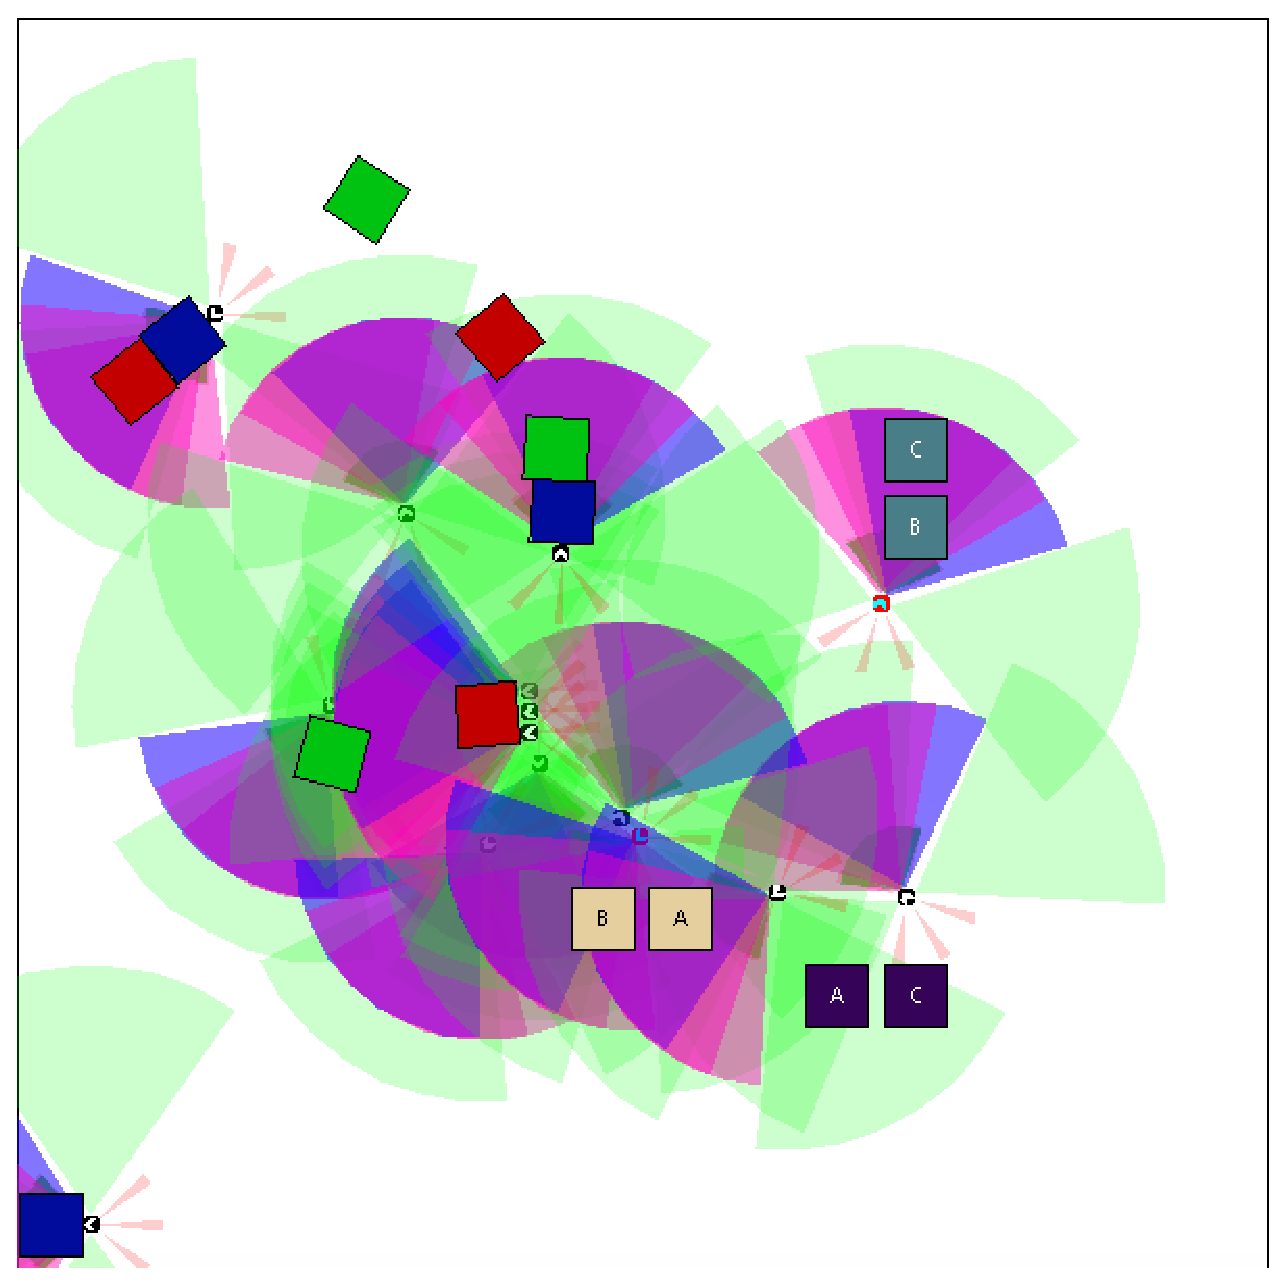
\includegraphics[width=0.40\textwidth]{TaskEnv.eps}
\caption{Example of the simulation environment.  Robots search for randomly distributed
type A, B, and C blocks (blue, green and red, respectively).  Other colored and labeled
blocks indicate those already connected in construction zones.
Different coloured semi-circles emanating from each
robot represent the field of view of currently active different sensor types (table \ref{tab:simParameters}).}\label{fig:taskEnv}
\end{figure}




\section{Simulated Environment}

These experiments were conducted in a simulated 2-dimensional environment that made use of the Redbridge simulator {insert a reference}

The robots that were used were simplified and abstracted versions of the Khepera robots (maybe find an online reference to what they are). This because they are relatively simple and cheap to buy and they are also compatible with a wide range of sensors.

The physics of the simulated environment were relatively basic. It was implemented by using the JBox2D library for Java.

The environment through which the agents move and in which they interact is continous space but the environment results are evaluated using an underlying discretised grid. This is also used to 'snap' the connected resources to a fixed location on the grid once it has been attached to the construction zone. This is determined by checking the resource's distance to a connection surface as well as the its orientation relative to the target bloc. If it is within an acceptable range, the block automatically snaps into place and becomes fixed in space.

This toolkit is written in Java and it was chosen because of its consistent performance across a range of machines and its compatibility with various operating systems which would be useful in the testing phase as we had to run the simulations on a number of machines.

One of the reasons for choosing the MASON Java library is because it can easily be integrated with other Java-based tools, such as the Encog Machine Learning library, which is discussed earlier on in this section (\ref{sec:method_hyperneat}).

\subsection{Construction Zone}

A construction zone refers to an already existing structure that consists of two or more connected resources.
Some examples of construction zones are shown in the following diagram (insert an illustration) and are indicated by the connected blocks changing to the same colour as well as having a label indicating the blocks type.

This is a collection of already constructed resources. It can be thought of as the current object that is currently under construction. This is the structure to which new resources should be connected in order to accomplish the construction of a single cohesive object rather than just a bunch of small structures that consist of 2 or 3 blocks.

Once a resource has been connected to a construction zone it becomes fixed in place. The entire construction zone is static and once a resource has been connected to it, it can not be disconnected again.

In order to encourage the construction of a single structure rather than just scattered structures that consist of 2 or 3 connected blocks, we restricted the number of construction zones to 3 per simulation. This means that 2 'free' resources can only be connected to each other thrice, the rest of the (subsequent) resources must be connected to one of those existing construction zones 
'This only gets done for the first three pairs of blocks in order to encourage the development of a singular structure instead of several smaller ones'

The fact that the construction zones are only created by whichever 2 resources are connected first means that the location of the construction zone is different for each simulation run and depends on where the robots connect the first 2 blocks.

\subsection{Resource Blocks}

In order to represent the raw materials that are scattered throughout the environment for which the agents must search, we made use of basic squares with different physical properties.

These properties include:
-> How many robots need to cooperate in order to be able to move the construction block
-> Which types of blocks can be connected on which specific sides of the construction block (these are referred to as the underlying construction schema).

Three different types of construction blocks were implemented in order to define the complexity/difficulty of the task at hand

The complexity of the task is defined by the simulated environment and the resources that are present within it.

\subsection{Construction Rules / Task Complexity}

The level of required cooperation and the complexity of each experiment is determined by the types of blocks present in the environment (cooperation to move heavier blocks) and whether or not there are any construction rules present in the current schema.

An illustrated example of how the various difficulty levels are implemented is shown in figure \ref{fig:constructionSchema}.
Additionally, these configurations are outlined in more details later on in table \ref{tab:taskComplexity}.

(Used to implicitly define the complexity of the simulated task at hand by controlling the simulated environment)

The connection schema specifies the number of each type of construction block that is to be placed in the environment for a specific experiment level. 

\begin{figure}[t]
	\centering
	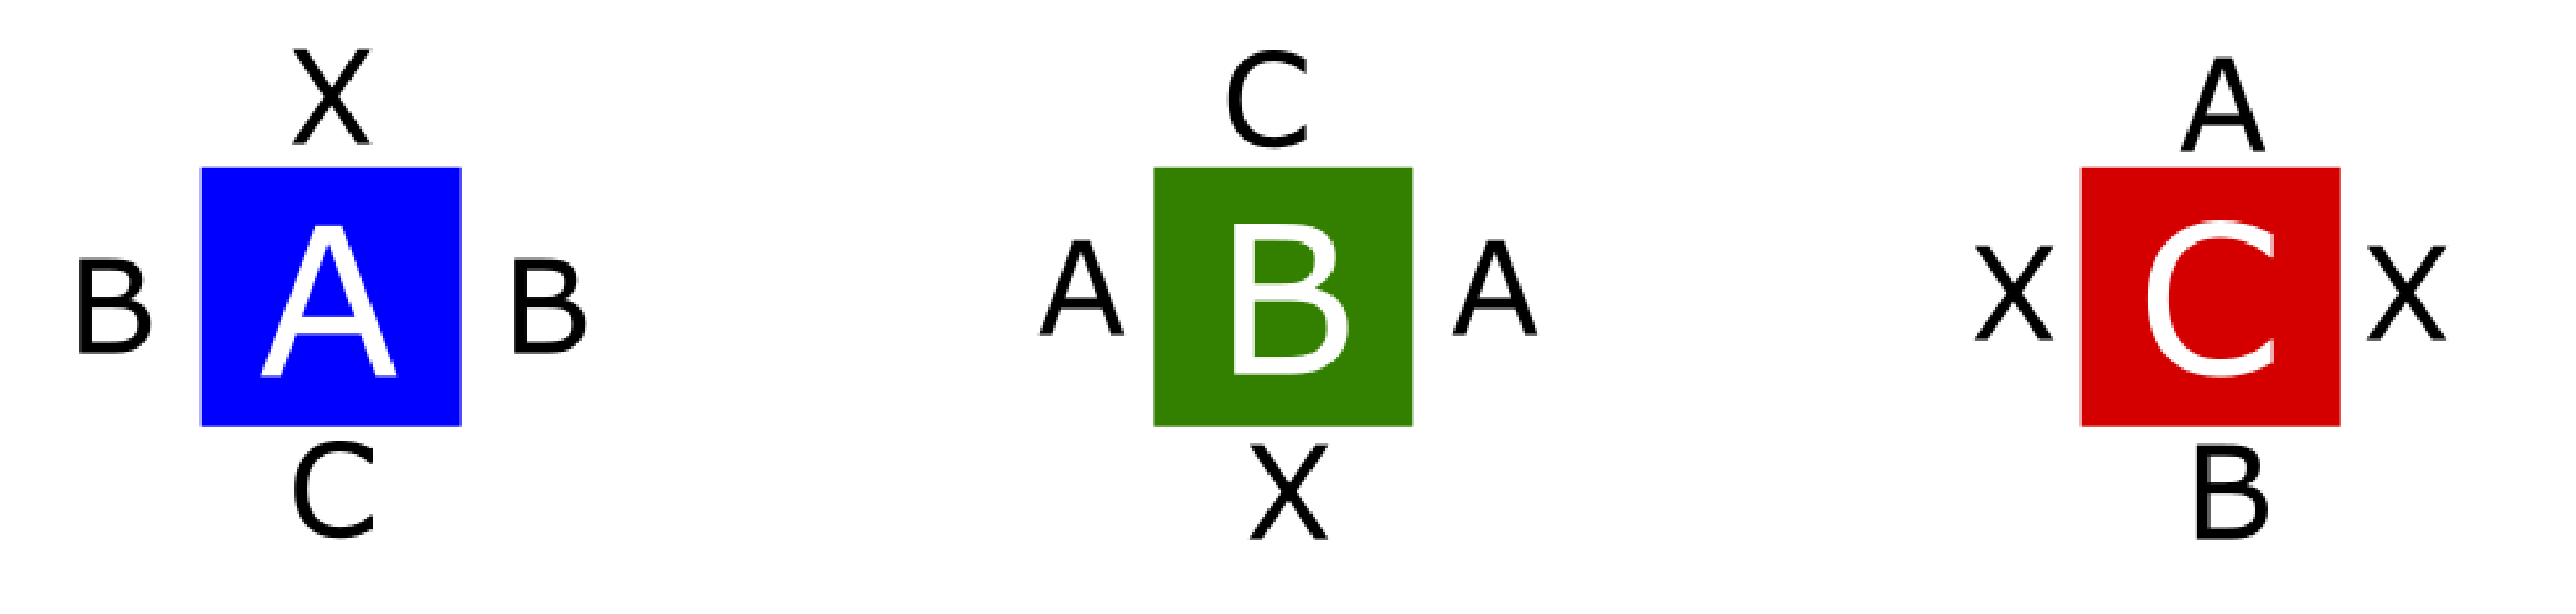
\includegraphics[width=0.5\textwidth]{ConstructionSchema.PNG}
	\caption{Task level 3 construction schema: \textit{A}, \textit{B}, and \textit{C} are the block types.  The label on
each side of each block type indicates what block type can be connected to this side.  An \textit{X} label indicates
that no block can be connected.}\label{fig:constructionSchema}
\end{figure}

Figure \ref{fig:constructionSchema} provides an illustrated version of the various types and numbers of resource blocks that are present for each experiment level.

Level $1$ was the least complex as it did not require
any cooperation, given that in this case there were only type \textit{A}
blocks in the environment.

Level $2$ was of medium complexity as there are equal numbers of type \textit{A},
\textit{B}, and \textit{C} blocks in the environment, where block types \textit{B} and \textit{C} required
at least two and three robots to push, respectively.

Level $3$ was the most complex, as it required the same degree of cooperation as task level
$2$, though blocks had to be connected according to a construction schema.
Figure \ref{fig:constructionSchema}
illustrates this construction schema, where the label on each of the
four sides of each block type indicates what other block type can be connected to the given side.

When block types have no letters on the sides it means that there were no blocks of that type present in the environment for that complexity level of the simulation (as with block types B and C in the first level of the illustrated schema)

\section{Collective Construction Task}

\hl{should this section not perhaps be part of the introduction section}

The collective construction task was chosen as it is a task that benefits from autonomous robot groups that must exhibit robust collective behaviour in dynamic, noisy environments. Also, the collective construction task includes the notion of morphological damage to robots that may impede group task accomplishment. 

The collective construction task requires that a team of agents cooperate by coordinating their behaviours in order to assemble various structures within their environment [reference] <verbatim from the honours paper>
In this case, a team of homogeneous robots needs to search for various types of construction block scattered throughout the environment and connect them in order to construct a single large structure. 

The collective construction task can be sub-divided into three smaller sub-tasks:
	First:
		the robots need to search the environment in order to find the loose construction blocks.
	Second:
		once a robot has located a block, it needs to pick it up and move it towards a construction zone. If there is no previously existing/created construction zone, then it needs to move the block towards another block in order to start a new construction zone. A new construction zone is created when any 2 free resources are successfully connected.
	Third:
		the robot must then try to connect the block it's carrying either to an existing construction zone or another block (to start a new construction zone). Once the robot has succcessfully connected the block to a construction zone, it releases the block and starts the process again by searching for another free block.

The robots need to cooperate in order to collect and construct the heavier block types.

The controller also needs to learn the underlying connection rules specified by the schema in order to be able to connect the appropriate block types to each other.




\subsection{Task Complexity}

The complexity of the collective construction task is controlled by implementing the different connection schemas. By requiring the robots to cooperate in order to be able to move certain block types and implementing connection rules, it is necessary to evolve more complex controllers that are able to account for cooperative interactions which is a non-trivial task for most Evolutionary Algorithms (should maybe find a reference for this past paragraph? Currently its taken straight from page 5 of honours paper)

The controllers that were produced using HyperNEAT and the various fitness functions were evaluated based on how successful they were at solving the collective construction task. A controller's task performance is defined by the number of different types of blocks that it managed to connect to a construction zone.

Each of the different types of construction blocks are worth a different score depending on what level of cooperation they require (how many agents it takes to move the block)
"I dont think there is any reward calculation for the complexity of the construction schema" The point is to simply deploy the agents with a more complex schema and then just see if they are able to solve the same task. I dont think its necessary to account for the difficulty level of the simulation in the fitness function calculation.

\subsection{Construction Schema}

The complexity/difficulty of a given simulation level is determined by the types of construction blocks present in the environment (as this determines the level of cooperation) as well as then underlying connection rules that govern which blocks can be connected to which other blocks and on their corresponding sides.

These underlying connection rules are specified using what will be referred to as a construction schema. This is essentially just a YAML file that indicates what block types can be attached to which side of each respective block. Whenever the robots attempt to connect 2 construction blocks, the simulator refers to this file and checks that the construction schema allows for these blocks to be connected on the indicated sides.

This is almost like an abstract representation of how receptors and hormones work in the brain, i think. Or is it something to do with DNA replication? Eitrher way, its like the lock-key model for proteins

This is analogous to the way in which puzzle pieces only fit together on specific sides and orientations.

When a robot attempts to attach 2 blocks to each other, the connection rules for both blocks must be satisfied in order for a successful connection to be made.


\section{Team Controller}

'This is from the GECCO Penultimate paper pg2, remember to go get the references and the diagrams'

Each robot's ANN controller comprised N sensory input and hidden nodes, connected hidden layer to two motor outputs (controlling the robot's left and right wheels). Nodes were arranged as a substrate where the number of input and hidden nodes was determined by a give robot morphology. Each substrate node was placed at specific (x,y) locations in the substrate's two-dimensional geometric space. Sensor nodes of the substrate approximated up to a 360deg sensory FOV, where the FOV was dependent on the morphology used.
































%\chapter{Experiments}
\label{Chapter4}


%%%%%%%%%%%%%%%%%%%%%%%%%%%%%%%%%%%%%%%%%%%%%%%%%%%%%%%%%%%%%%%%%%%%%%%%%%%%%%%%%%%%%%%%%%%%%
%% From the SSCI Paper -> HyperNEAT Objective (Fixed morph, sets of morphs, random morphs) %%
%% This works out to the same as the 4 sets of morphologies and the fifth variable one	   %%
%% HyperNEAT Objective
%% 4 Morphs and 1 variable

%SSCI -> HyperNEAT objective across 5 morphologies and 3 complexity levels

\section{Experiment Outline} \label{sec:experiment_outline}

Experiments were used to evaluate the \textit{morphological robustness} of ANN controllers evolved using the HyperNEAT algorithm for
robot teams that must accomplish a collective construction task of increasing
complexity (section \ref{subsec:constructionTask}).

We measured the average comparative task performance of controllers evolved
for a given team morphology and task complexity (this is calculated during the 'Baseline' step) where such controllers were
then transferred to
and re-evaluated across other team morphologies.

Thus, teams that achieved an average task performance that was not significantly lower
across all \textit{re-evaluated} morphologies were considered to be \textit{morphologically robust}.

This study comprised five experiment sets, where the first four experiment sets evolved
controllers given team morphologies $1-4$ (table \ref{tab:morphConfigs})
for three levels of increasing task complexity (table \ref{tab:taskComplexity}).

The fifth experiment set investigated the \textit{co-adaptation} of team morphology
and behavior, where morphology $5$ (table \ref{tab:morphConfigs}) was used
as the initial sensory configuration for all robots in the team.

This fifth experiment set was included in order to gauge if co-adapting behavior
and morphology yielded any benefits in this collective construction task as it did in related
collective behavior tasks \cite{HewlandNitschke2015}.

Each experiment set \footnote{Source code for all experiments is online at: \url{https://github.com/not-my-name/ExperimentsRerun}} tested a team of $15$ robots in a bounded ($20$ x $20$ units), two-dimensional, and continuous simulated environment along with a collection of randomly distributed resource blocks of type \textit{A}, \textit{B}, and \textit{C} (table \ref{}tab:simParameters).

During initialization of an experiment run, the robots and the resource blocks were placed at random locations and with random orientations.

A construction schema (table \ref{tab:taskComplexity}) dictated the sequence of block
types that must be connected together in order that a specific structure be built \cite{NitschkeSaEC2012}.

Figure \ref{fig:taskEnv} presents an example of the team of $15$ robots working to solve the
collective construction task in the simulation environment containing a distribution of five of each
block type (\textit{A}, \textit{B} and \textit{C}), colored blue, green and red, respectively.
Other colored blocks in the environment indicate those already connected in construction zones
(three illustrated).  

The purple, blue and green semi-circles emanating from each robot
represent the FOV of active sensors, where the different colors correspond to different
sensor types (table \ref{tab:simParameters}).

As the purpose this study was to demonstrate the morphological robustness of
HyperNEAT evolved controllers for a collective behavior task of increasing complexity,
the first two versions of the collective construction task required no cooperation and some degree of
cooperation, respectively, though any block could be connected to any other block.
Where as, the most complex version of the task required cooperation and block types
to be connected according to a construction schema (table \ref{tab:taskComplexity})

The fittest controller evolved for each experiment set (yielding the highest absolute task performance)
was then \textit{evaluated} for morphological robustness across all other morphologies.

For example, the fittest controller evolved for morphology $1$ was evaluated across morphologies
$2-4$ and the average task performance calculated across all evaluation runs.
%($1$ to $7$ in table \ref{tab:morphConfigs}) for the given task.

Each set of experiments (testing conditions?) can be broken into the following distinct stages:
1] Evolution 
2] Baseline Calculation
3] Evaluation

\hl{The above steps are repeated for each set of experimental conditions, namely the objective and novelty fitness functions. On a similar note, the novelty search function was only tested on a smaller subset of the predefined morphologies (this was due to time and resource constraints)}


\subsection{Evolution Phase}

For controller evolution, each experiment applied HyperNEAT to evolve team behavior for
$15$ robots over $100$ generations,
where a generation is comprised of $5$ \textit{team lifetimes} (with $1000$ simulation iterations per lifetime).

A single evolution phase can broken down into the following distinct steps:
1] Simulation - The team of agents are deployed into the simulated environment along with the necessary resource blocks. The agents must then operate within this environment for a 'lifetime', attempting to solve the task at hand.  A single 'Simulation' step consists of $5$ lifetimes,
2] Fitness Calculation - At the end of each lifetime, the environment is analysed and compared with the desired output. At the end of a 'Simulation' step, the fitness of the controller is calculated using an average of these values and the provided fitness function. This value indicates a controller's suitability to solving the collective construction task.
3] HyperNEAT Evolution - The fitness scores obtained in the previous steps are passed to the Evolutionary Algorithm (along with their respective controllers) at which point the subsequent generation of controllers are created

Each team lifetime tested different robot starting positions, orientations, and block locations
in the simulation environment.


\subsection{Baseline}

The purpose of this stage is to simply calculate an accurate average fitness score for each optimal controller. This average fitness provides a more accurate indication of a controller's suitability to solving the task.

During this simulation stage, the parameters are the same as for the evolution phase in which the controller was evolved (ie. the same length of lifetime (simulation steps), same block configuration, same construction schema).

In order to obtain this 'baseline' average score, the absolute fittest controller for each experimental condition is redeployed in the simulator and allowed to try and solve the task. 

A single 'baseline' attempt in the simulator is equivalent to $1$ team lifetime and this is repeated for $20$ lifetimes and an average fitness score is calculated.

During this stage, no Machine Learning processes or evolutionary steps are performed.

\subsection{Evaluation}

Each evaluation run was \textit{non-evolutionary}, where controllers were not further evolved,
and each evaluation run in the simulator was equivalent to one team lifetime.

Evaluation runs were repeated $20$ times for a given morphology, in order to account for random variations in robot and block
starting positions and orientations.

For each fittest controller, evaluated in a given morphology, an average baseline task performance was
calculated over these $20$ runs, and then an overall average task performance was computed across all evaluated morphologies, producing an average fitness score that indicated a particular controller's ability to adapt to changes in its sensory configuration (morphology).

As per this study's objectives, these morphological re-evaluation
runs tested how robust the fittest evolved controllers (for a given morphology) were to variations
in that morphology.
Thus, re-evaluating the fittest controllers on other morphologies emulated sensor loss due
to damage or new robot morphologies introduced due to changing task constraints.


%%%%%%%%%%%%%%%%%%%%%%%%%%%%%%%%%%%%%%%%%%%%%%%%%%%%%%%%%%%%%%%%%%%%%%%%%%%%%
%% This is the table from the SSCI paper.								   %%	
%% Just be sure to double check that the values are correct for all of     %%
%% the experiments that are included in this paper (across AAMAS and SSCI) %%
%%%%%%%%%%%%%%%%%%%%%%%%%%%%%%%%%%%%%%%%%%%%%%%%%%%%%%%%%%%%%%%%%%%%%%%%%%%%%

\begin{table}
	\renewcommand{\arraystretch}{1.30}
	\caption{Experiment, Neuro-evolution and Sensor Parameters}\label{tab:simParameters}
	\centering
	\begin{tabular}{llc}
		\hline
		Generations	                                           & 100	\\
		Sensors per robot                                      & 11, 8, 4, 6, random \\	
		Evaluations per genotype                               & 5  \\
		Experiment runs                                        & 20 \\
		Environment length, width                              & 20 \\
        Max Distance (Robot movement per iteration)            & 1.0 \\
        Team size                                              & 15 \\
        Team Lifetime (Simulation iterations)                  & 1000 \\	
        Lifetimes per generation                               & 5 \\
        Type A blocks (1 robot to push)                        & 15 \\
        Type B blocks (2 robots to push)                       & 15 \\
        Type C blocks (3 robots to push)                       & 15 \\
		\hline
		\multirow{4}{*}{Mutation rate} & Add neuron            & 0.25 \\
		& Add connection                                       & 0.008  \\
		& Remove connection                                    & 0.002 \\
		& Weight                                               & 0.1  \\
		Population size                                        & 150 \\
		Survival rate                                          & 0.3 \\
		Crossover proportion                                   & 0.5 \\
		Elitism proportion                                     & 0.1 \\
		CPPN topology                                          & Feed-forward           \\
		CPPN inputs                                            & Position, delta, angle \\
		\hline
		Sensor                                                 & Range     & FOV \\
		\hline
		Proximity Sensor		                               & 	1.0	   &  0.2  \\
		Ultrasonic Sensor		                               &	4.0    &  1.2  \\
		Ranged Colour Sensor	                               &	3.0	   &  1.5 \\
		Low-Res Camera			                               & 	3.0	   &  1.5 \\
		Colour Proximity Sensor                                & 	3.0	   &  3.0 \\
		\hline
	\end{tabular}
\end{table}



%%%%%%%%%%%%%%%%%%%%%%%%%%%%%%%%%%%%%%%%%%%%%%
%% Below table is from the SSCI experiments %%
%%%%%%%%%%%%%%%%%%%%%%%%%%%%%%%%%%%%%%%%%%%%%%
\begin{table}[t]
	\renewcommand{\arraystretch}{1.30}
	\caption{Task Complexity. Note: Task level 3 includes a construction schema (figure \ref{fig:constructionSchema}).}\label{tab:taskComplexity}
	\centering
	\begin{tabular}{lccc}
		\hline
		Construction Task Complexity                               & Level 1     & Level 2    & Level 3   \\
		\hline
		Type A blocks (1 robot to push)	                           & 	15	     & 5          & 5  \\
		Type B blocks (2 robots to push)		                   &	0 	     & 5          & 5  \\
		Type C blocks (3 robots to push)	                       &  	0	     & 5          & 5  \\
		Construction schema                                        &   No        & No         &	Yes \\
\hline
	\end{tabular}
\end{table}

The above table shows the overall outline for the resources used across the various experiments.
For the experiments that did not make use of all of the resources listed above, they simply used a subset 
of the above resources.




 
%\chapter{Results \& Discussion}
\label{Chapter5}

		%%%%%%%%%%%%%%%%%%%%%%%%%%%%%%%%%%%%%%%%%%%%%%%%%%%%%%%%%%%%%%%%%%%%%%%%%%%%%%
		%%				Results and Discussion From AAMAS Abstract					%%
		%%			Experiments Compared With Objective and Novelty Search			%%
		%%	Will need to make sure to include the correct results graphs and plots	%%
		%%%%%%%%%%%%%%%%%%%%%%%%%%%%%%%%%%%%%%%%%%%%%%%%%%%%%%%%%%%%%%%%%%%%%%%%%%%%%%

Results indicate that, for both novelty and objective search, given increasing task complexity, there was no significant difference in average task performance between the controllers evolved in any morphology and then evaluated in other morphologies.

However, there were two exceptions to this result. 
First, novelty search applied in task complexity level 1 to evolve controllers evaluated in morphology 3 yielded significantly lower average task performance.

Second, objective search applied in task complexity level 2 to evolve controllers in morphology 1, where similarly, the fittest controller evaluated in morphology 3 yielded a significantly lower task performance.

In these cases, one may observe that there is a large difference in the number of sensors used by morphology 1 versus morphology 3 (table from AAMAS Abstract), indicating that controllers evolved for the high sensory complement (and thus functionality) of morphology 1 are not readily transferable to a simpler sensory configuration (with much less functionality). 

However, this was not the case for novelty search applied in task level 2 or objective-search  applied in task level 1.

The key results were thus two-fold. 
First (supporting the first hypothesis), team behaviours evolved by novelty search, for ALL morphologies and task complexity levels, significantly out-performed team behaviours evolved with objective search for corresponding morphologies and task complexity levels. 
	This result is supported by the following previous work 
		\cite{DidiNitschke2016SSCI}, 
		\cite{DidiNitschke2016},
		\cite{gomes2013generic},
		\cite{RefWorks:5},
		\cite{RefWorks:11}

Second (refuting the second hypothesis), results indicated that, for all team morphologies and levels of task complexity evaluated, both novelty and objective search were effective in evolving morphologically robust controllers.

That is, for any given morphology, there was no significant difference in average task performance between the fittest novelty search evolved controllers and "re-evaluation" of these controllers in the other morphologies. 

The same result was observed for objective search.
This second result indicates that while novelty search yields advantages over objective search in terms of evolving high task performance team behaviours, it yields no benefits over objective search for evolving morphologically robust controllers in the collective construction task for the given team morphologies.
However, the suitability of novelty search for evolving morphologically robust controllers in complex collective behaviour tasks is the topic of ongoing research.

%%%%%%%%%%%%%%%%%%%%%%%%%%%%%%%%%%%%%%%%%%%%%%%%%%%%%%%%%%%%%%%%%%%%%%%%%%%%%%%%%%%%%%%%%%%%%%%




%%%%%%%%%%%%%%%%%%%%%%%%%%%%%%%%%%%%%%%%%%%%%%%%%%%%
%%				From the GECCO Draft			  %%
%% 			   Results and Discussion			  %%
%%			Objective VS Novelty Search			  %%
%%%%%%%%%%%%%%%%%%%%%%%%%%%%%%%%%%%%%%%%%%%%%%%%%%%%

To address the research objectives, we compared the average task performance results of team behaviour evolution directed by objective versus novelty search. 
For each experiment, task performance was the number of blocks connected in construction zones over a team's lifetime, where the maximum task performance was taken at each run's end and an average task performance calculated over 20 runs (the "Evaluation Phase").


%%%%%%%%%%%%%%%%%%%%%%%%%%%%%%%%%%%%%%%%%%%%%%%%%%%%








\begin{figure*}[t]
	\begin{minipage}{0.5\textwidth}
		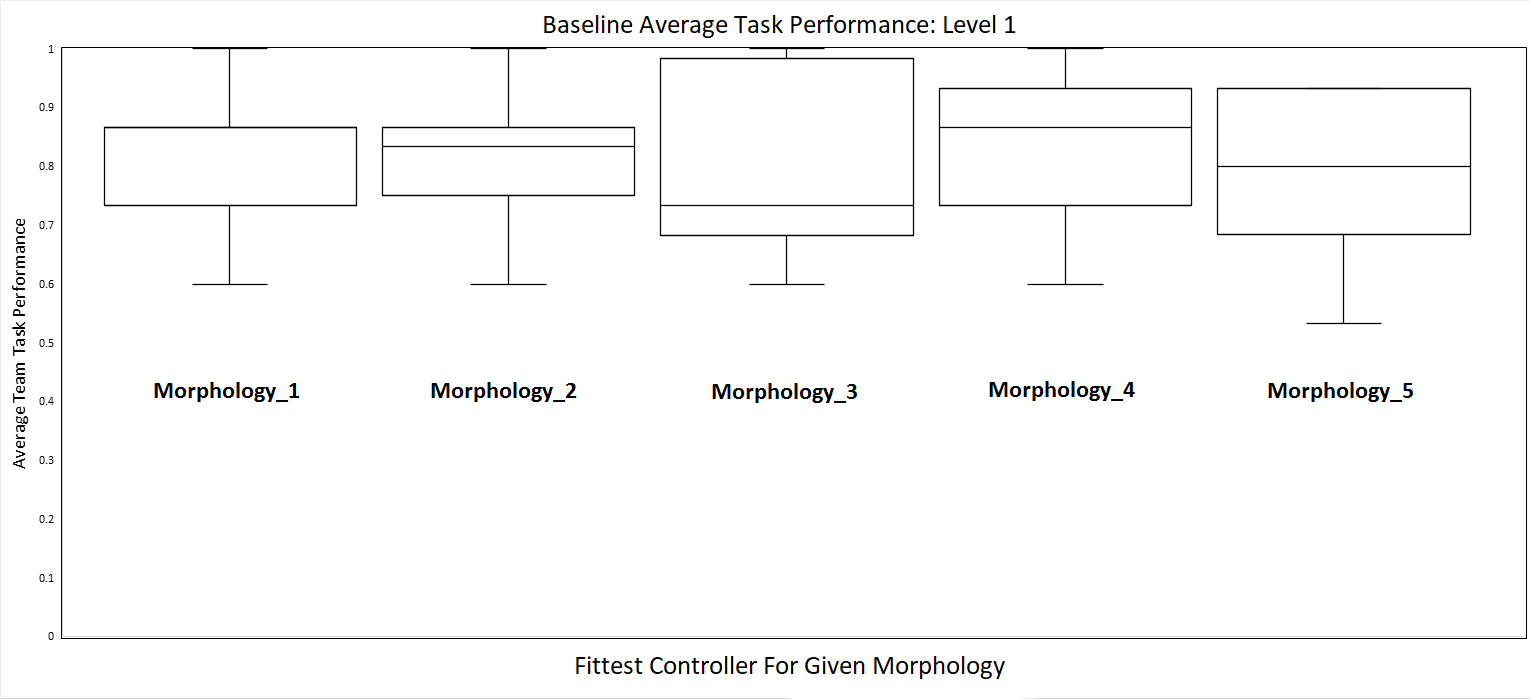
\includegraphics[width=\textwidth]{Baseline_Level_1.png}
	\end{minipage}
	\begin{minipage}{0.5\textwidth}
		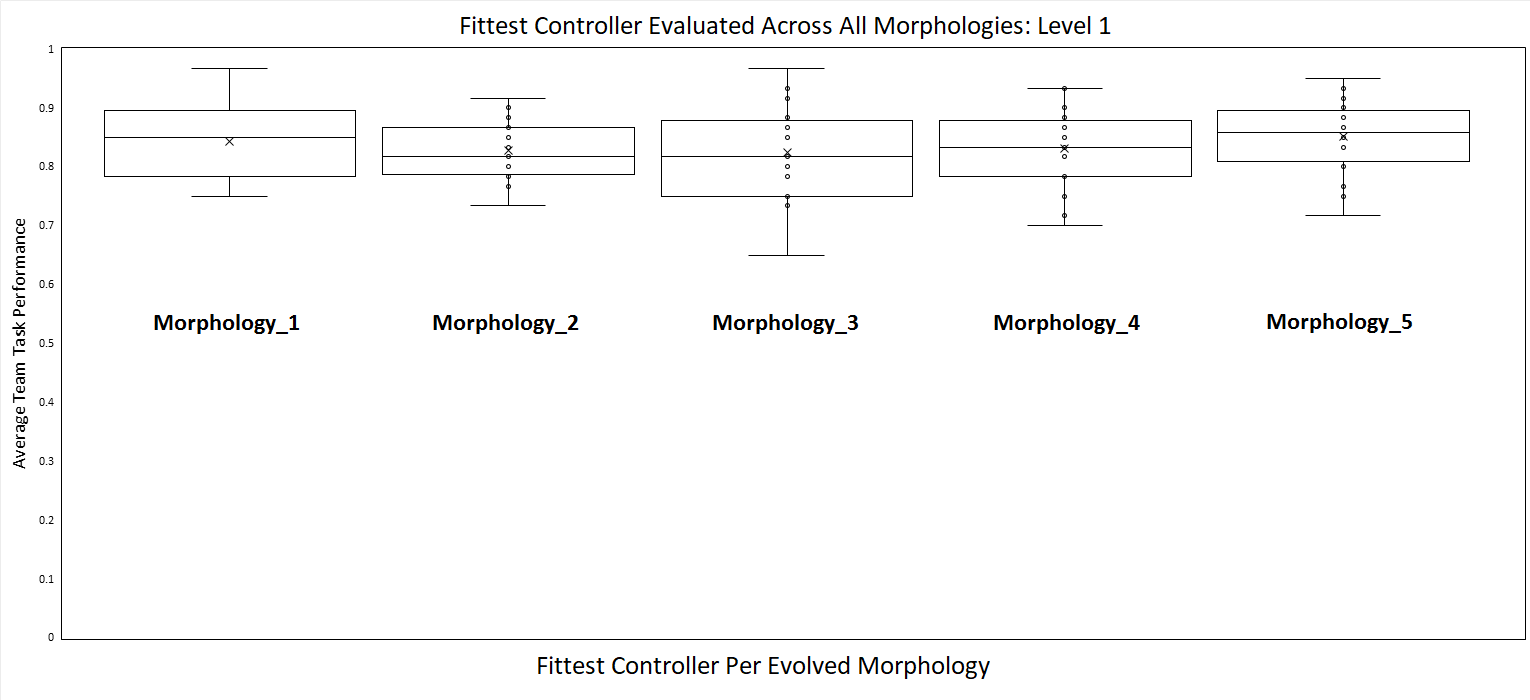
\includegraphics[width=\textwidth]{Average_Eval_Level_1.png}
	\end{minipage}
\caption{\textit{Left column:} Baseline task performance for evolved controllers (\textit{task level 1})
given morphologies $1-5$ (depicted from left to right).
\textit{Right column:} Average task performance given the fittest controller evolved
for each respective morphology ($1-5$, shown left to right) evaluated across all other morphologies.
For example: Left-most plot is average task performance of fittest controller evolved for
morphology $1$, evaluated across morphologies $2-5$.  Right-most plot is the average task performance
of fittest controller evolved for morphology $5$, evaluated across morphologies $1-4$.}\label{fig:level1results}
\end{figure*}

\begin{figure*}[t]
	\begin{minipage}{0.5\textwidth}
		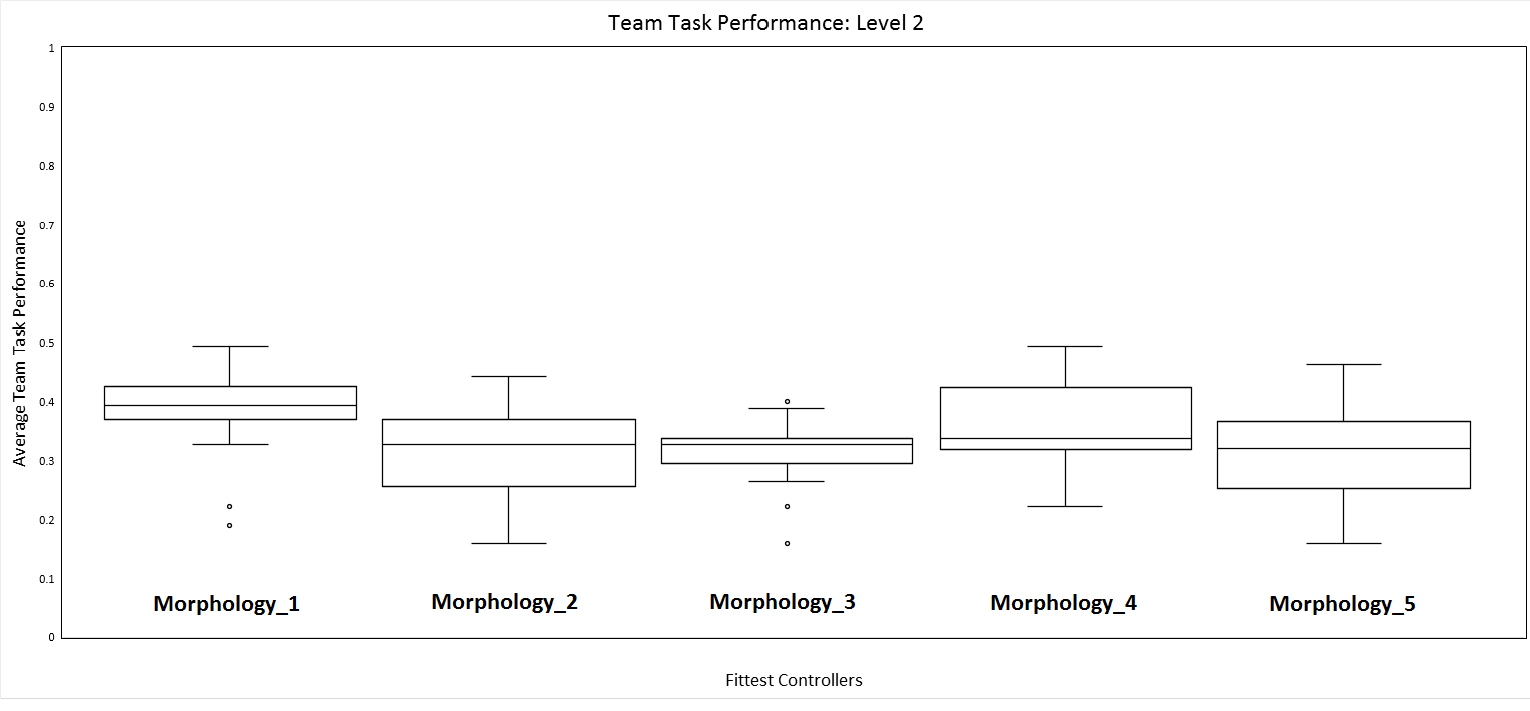
\includegraphics[width=\textwidth]{Baseline_Level_2.png}
	\end{minipage}
	\begin{minipage}{0.5\textwidth}
		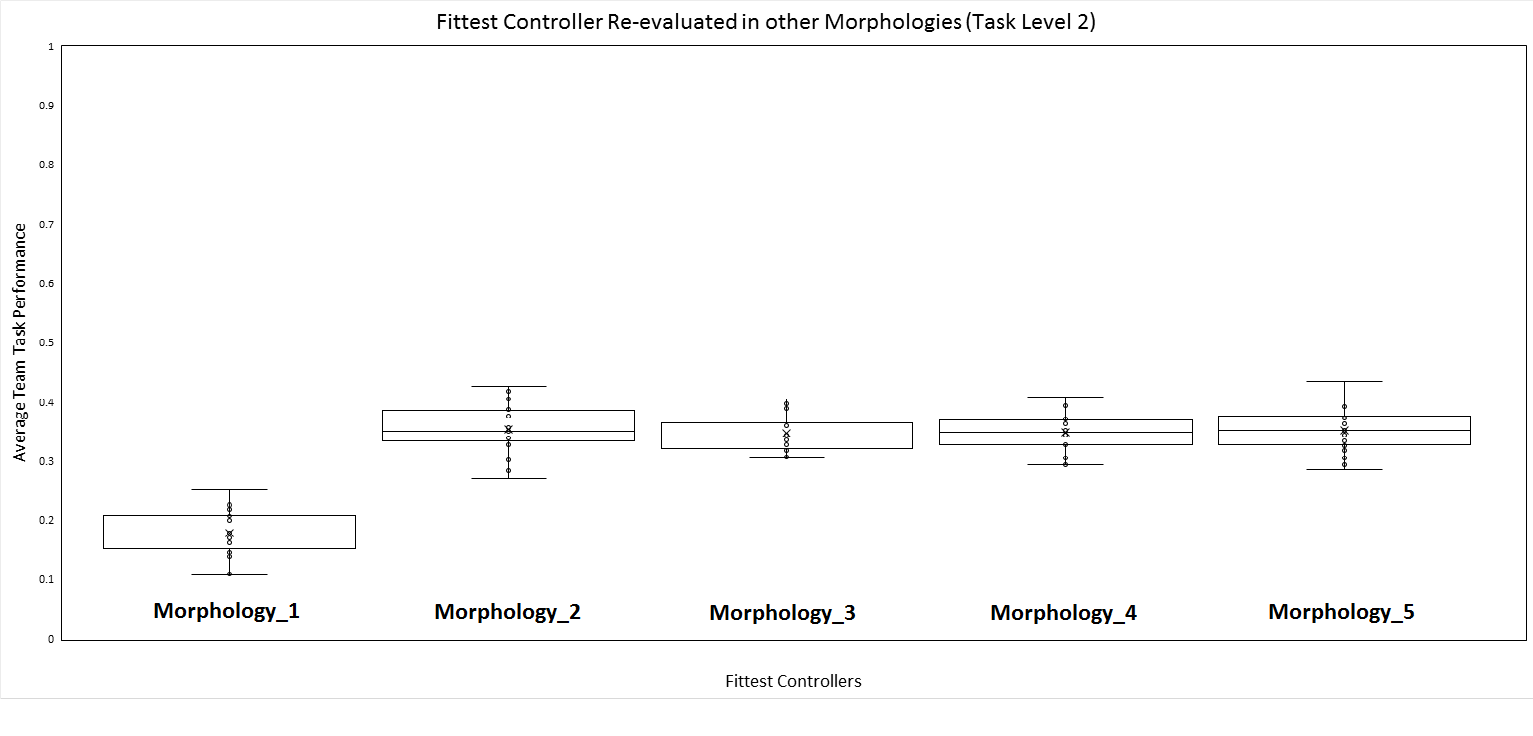
\includegraphics[width=\textwidth]{Average_Eval_Level_2.png}
	\end{minipage}
\caption{\textit{Left column:} Baseline task performance for evolved controllers (\textit{task level 1})
given morphologies $1-5$ (depicted from left to right).
\textit{Right column:} Average task performance given the fittest controller evolved
for each respective morphology ($1-5$, shown left to right) evaluated across all other morphologies.
For example: Left-most plot is average task performance of fittest controller evolved for
morphology $1$, evaluated across morphologies $2-5$.  Right-most plot is the average task performance
of fittest controller evolved for morphology $5$, evaluated across morphologies $1-4$.}\label{fig:level2results}
\end{figure*}

\begin{figure*}[t]
	\begin{minipage}{0.5\textwidth}
		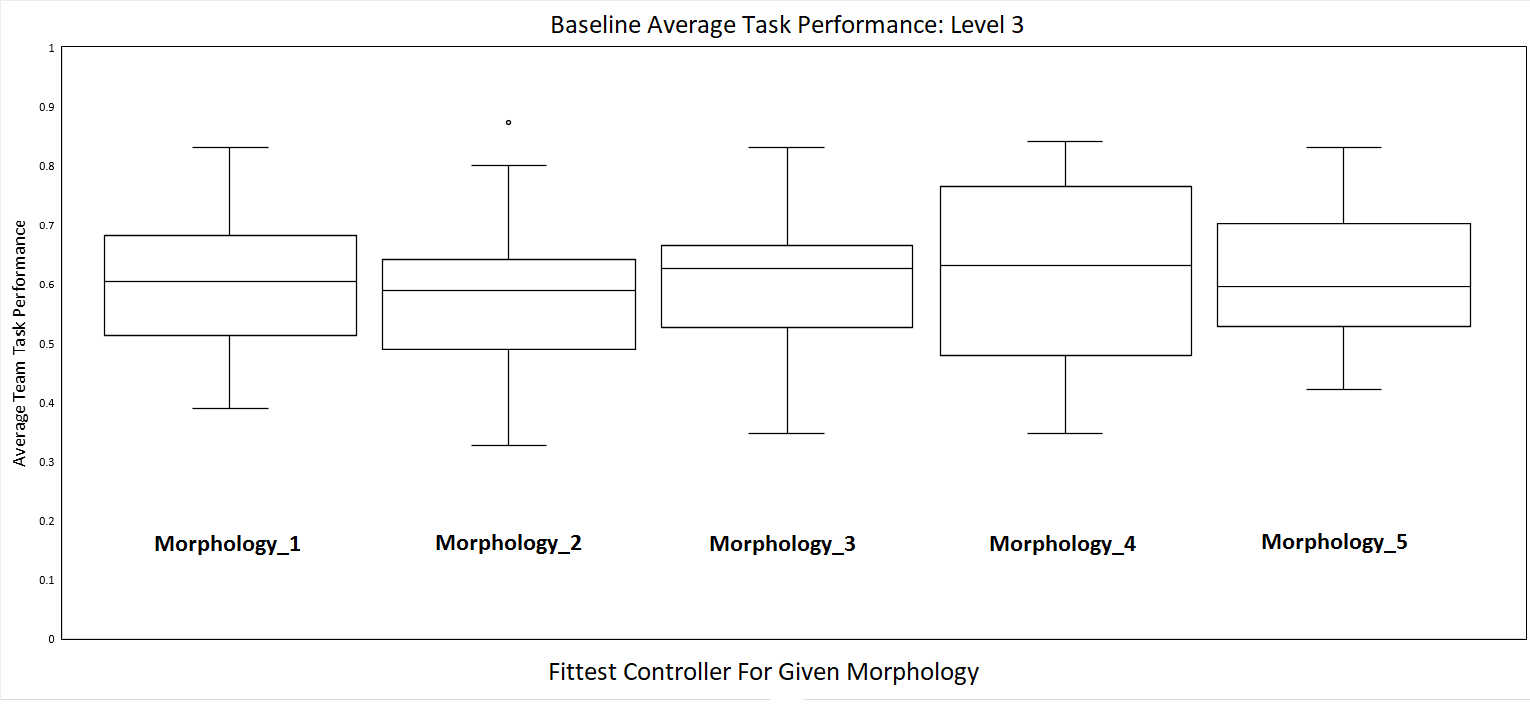
\includegraphics[width=\textwidth]{Baseline_Level_3.png}
	\end{minipage}
	\begin{minipage}{0.5\textwidth}
		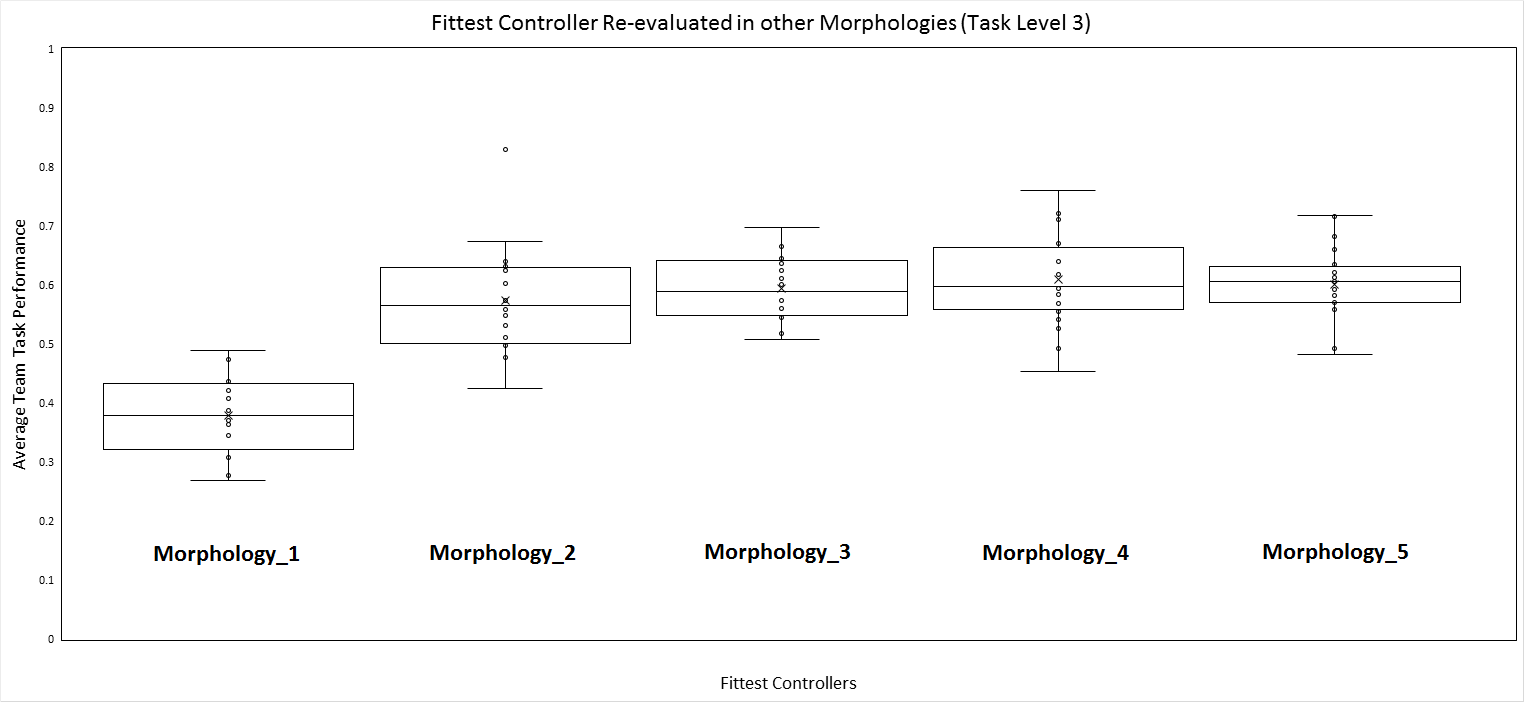
\includegraphics[width=\textwidth]{Average_Eval_Level_3.png}
	\end{minipage}
\caption{\textit{Left column:} Baseline task performance for evolved controllers (\textit{task level 1})
given morphologies $1-5$ (depicted from left to right).
\textit{Right column:} Average task performance given the fittest controller evolved
for each respective morphology ($1-5$, shown left to right) evaluated across all other morphologies.
For example: Left-most plot is average task performance of fittest controller evolved for
morphology $1$, evaluated across morphologies $2-5$.  Right-most plot is the average task performance
of fittest controller evolved for morphology $5$, evaluated across morphologies $1-4$.}\label{fig:level3results}
\end{figure*}


For each evolution phase of an experiment set, the average maximum task performance
of controllers evolved for a given morphology and level of task complexity, was recorded.

Specifically, this task performance was calculated by running the absolute fittest controller
evolved after $20$ evolutionary runs (for a given a morphology and task level),
in the same morphology over $20$ non-evolutionary runs (baseline calculations in \ref{sec:experiment_outline}).

This is previously referred to as the baseline average score for a specific controller (section \ref{sec:experiment_outline}).

This is presented in figures \ref{fig:level1results}, \ref{fig:level2results} and \ref{fig:level3results}
(left column), where controllers were evolved given morphologies $1$-$5$ (table \ref{tab:morphConfigs}).
In figures \ref{fig:level1results}, \ref{fig:level2results} and \ref{fig:level3results} (left column),
these results are presented from left to right.

For example, average task performance results for morphology $1$ are plotted on the left-most side
and average task performance results for morphology $5$ are plotted on the right-most side.

For each evaluation phase of an experiment set, the fittest controller evolved for a given morphology and task complexity
level was evaluated across all other morphologies (for the same level of task complexity), and an
average task performance computed over $20$ runs.

These morphological evaluation results are presented in figures \ref{fig:level1results}, \ref{fig:level2results}
and \ref{fig:level3results} (right column).

Each of the five plots (from left to right) in each figure corresponds to the fittest controller evolved for each of the
five morphologies and re-evaluated in all other morphologies.  
For example, the left-most plot presents
the average task performance of the fittest controller evolved in morphology $1$ and re-evaluated on morphologies $2-5$.

Where as, the right-most plot presents the average task performance of the fittest controller evolved given morphology $5$
(as the initial sensory configuration) and re-evaluated on morphologies $1-4$.

To gauge the impact of a given team morphology (table \ref{tab:morphConfigs})
in company with a given level of task complexity (table \ref{tab:taskComplexity}),
the \textit{t-test} \cite{FlanneryTeukolsky1986} ($p < 0.05$),
was applied in pair-wise comparisons between sets of controller evolution
results\footnote{Statistical test results for pair-wise comparisons for the fittest evolved controllers
(for a given morphology) tested in each other morphology (individually) is online at:
\url{https://github.com/not-my-name/SSCI_Paper_Appendix}}
(figures \ref{fig:level1results}, \ref{fig:level2results} and \ref{fig:level3results}, left column).

Within each given level of task complexity, no statistically significant difference was found between
controllers evolved given morphologies $1-5$ (controller evolution experiments $1-5$).

Controller evolution experiments $1-4$ were those implementing controller evolution in fixed sensory
configurations (morphologies $1-4$).  Where as, controller evolution experiment $5$ used morphology $5$
as the initial sensory configuration and subsequently co-adapted behavior (controller) and morphology
(complement of sensors).

The lack of statistical difference between controllers evolved given morphologies $1-4$ (table \ref{tab:morphConfigs})
indicates that these sensory configurations were not sufficiently different so as to result in
significantly different average maximum task performances.

Also, the lack of any significant difference between the average maximum task performance of controllers
evolved given morphologies $1-4$ and behavior-morphology co-adaptation (starting with morphology $5$),
supports previous results demonstrating that behavior-morphology co-adaptation
yields at least comparable task performance benefits (compared to fixed morphology controller evolution)
in collective behavior tasks \cite{HewlandNitschke2015}.

However, to address this study's main objective it was necessary to ascertain the morphological robustness
of the fittest controller evolved in each morphology when re-evaluated in all other morphologies.

To gauge the morphological robustness of the fittest controllers evolved for a given morphology ($1-5$),
and a given task complexity, we applied the t-test in pair-wise comparisons of two result
data sets.  

First, the average maximum task performances yielded by controller evolution in morphologies
$1-5$ and second, the average maximum task performances yielded from evaluating the fittest controller
evolved for a given morphology in all other morphologies (section \ref{subsec:expDesign}).
%Thus, we also used two-way ANOVA tests to measure the impact of task complexity and re-evaluating the fittest
%controller evolved for each morphology on all morphologies (in comparison to controller evolution results).

Statistical test results indicated no significant difference (with one exception) between average task performance results
yielded by baseline calculations and morphological evaluation experiments for all task complexity levels.

Specifically, the average maximum task performance yielded by controllers evolved given morphologies $2$-$5$
(figures \ref{fig:level1results}, \ref{fig:level2results}, \ref{fig:level3results}, left column) was not
significantly lower than the average task performance yielded by the fittest controllers
(evolved in morphologies $1-5$), and then re-evaluated on other morphologies
(figures \ref{fig:level1results}, \ref{fig:level2results}, \ref{fig:level3results},
right column).  

The exception was morphology $1$ in task complexity levels $2$ and $3$.

In these tasks, the fittest controller evolved for morphology $1$, yielded a significantly higher average
baseline task performance than that yielded when this fittest controller was evaluated in
morphologies $2-5$.

%Statistical test results are summarized in tables \ref{tab:anovaL1}, \ref{tab:anovaL2}
%and \ref{tab:anovaL3} for task complexity levels $1$, $2$ and $3$, respectively,
%and include performance results comparisons between controller evolution and
%morphological re-evaluation experiments with respect to task complexity and morphology.

Hence, these results indicate that controllers evolved by HyperNEAT for a given morphology
(table \ref{tab:morphConfigs}), overall have the capacity to continue to effectively operate
when transferred to other morphologies.

This result was found to hold for all four of the five morphologies that controllers were evolved for,
and for all levels of task complexity tested (table \ref{tab:taskComplexity}).
%thus demonstrating the morphological robustness of HyperNEAT evolved controllers.

The efficacy of HyperNEAT for evolving morphologically robust controllers is further supported
by the controller evolution experiments that used morphology $5$ (section \ref{sec:experiments}).

In this case, the number of sensors was adapted meaning that team behavior and
morphology were co-adapted.

Specifically, these controller evolution experiments began with the sensory configuration of
morphology $5$ (table \ref{tab:morphConfigs}) and enabled and disabled sensor connections to
better couple morphology with the evolved controller.  

Hence, the fittest controller evolved in this case often corresponded to a sensory configuration
dissimilar to morphology $5$ (the initial sensory configuration).

Results indicated that the fittest controller evolved for morphology $5$, when evaluated across
other morphologies, yielded an average task performance that was statistically comparable to
the average baseline task performance yielded given morphology $5$.

This result was observed for all three task complexity levels
(figures \ref{fig:level1results}, \ref{fig:level2results}, and \ref{fig:level3results}, right column).

Thus, controllers evolved for fixed morphologies ($1-4$, table \ref{tab:morphConfigs}), were
found to be \textit{morphologically robust}, as there was no significant difference in average maximum
task performance when the fittest controller (evolved for morphology $1-4$), was evaluated using other
morphologies.

Furthermore, the fittest controller evolved for an adaptive morphology ($5$, table \ref{tab:morphConfigs}),
was similarly found to be morphologically robust, given that the average maximum task performance
yielded when this fittest controller was evaluated in other morphologies ($1-4$), was comparable to
the average maximum task performance yielded from morphology $5$ controller evolution experiment (baseline average fitness).

This is theorized to be a result of the complexity of co-adapting effective controller-morphology
couplings \cite{PfeiferBongard2006} within limited periods of artificial evolution ($100$ generations in these experiments,
table \ref{tab:simParameters}), offset by the transference of evolved
\textit{connectivity patterns} \cite{GauciStanley2010} as functional controllers across varying
robot morphologies  \cite{RisiStanley2013}.

Such connectivity patterns encode behaviors that do not rely upon specific sensory-motor mappings in
controllers and thus do not necessitate specific task environment configurations,
such as specific numbers of agents or objects.

This in turn facilitates the transfer of controllers across varying team morphologies
\cite{verbancsics_evolving_2010}, \cite{DidiNitschke2016SSCI}, \cite{DidiNitschke2016}.
%a benefit of HyperNEAT elucidated from such collective behavior transfer research was found to be its capability
%to evolve connectivity patterns between the sensory-motor layers of agent controllers
%that are broadly applicable to collective behavior tasks of varying complexity.
%versus adaptive morphologies had no significant impact on the
%morphological robustness of HyperNEAT evolved controllers (gauged in terms of average team task performance)
%for all morphologies tested.  %This result was observed for all levels of task complexity tested.

These results are corroborated by related work \cite{RisiStanley2013}, \cite{WatsonNitschke2015SSCI},
and contribute further empirical evidence that HyperNEAT yields significant benefits in
evolving robot controllers that effectively operate in other morphologies.

That is, this study further demonstrated HyperNEAT's capability to exploit geometric properties
such as regularity, repetition and symmetry in robot morphology and environment \cite{StanleyDAmbrosioGauci2009},
where such modularity and geometric properties are encoded in evolved connectivity patterns.

This is prevalent in this study, as the configuration of sensors on each robot's periphery was
symmetrical for all morphologies tested (section \ref{sec:embodiment}).
\hl{Not sure if the above is correct since Morph 5 was a random distribution}


Also, the collective construction task required that blocks be connected together in a repeated manner in a symmetrical bounded
simulation environment ($20$x$20$ units, table \ref{tab:simParameters}).

The capability of HyperNEAT evolved controllers to operate in different morphologies is further
supported by other research \cite{verbancsics_evolving_2010}
demonstrating that evolved indirect sensory-motor mappings can
encapsulate effective behaviors with relatively few task environment and robot
geometric relationships, such as desired positions and angles between robots and different object types.

The efficacy of HyperNEAT for evolving morphologically robust controllers for collective behavior
tasks of varying complexity is also supported by related research in \textit{multi-agent policy transfer}
\cite{verbancsics_evolving_2010}, \cite{DidiNitschke2016SSCI}, \cite{DidiNitschke2016}.

Policy transfer methods facilitate the transfer of behaviors across tasks of increasing
complexity or between dissimilar tasks.  

Such studies have demonstrated that HyperNEAT is an effective
method for evolving behaviors in one collective behavior task and then transferring the evolved behavior
to a related but more complex task (for example, where robots have more complex sensory-motor configurations
to process increased task complexity) with relatively little loss in average team task performance.
%That is, HyperNEAT evolves CPPNs representing controllers of varying complexity with their own symmetries
%and regularities which are able to effectively exploit varyingly complex robot (agent) sensory-motor configurations.
%This in turn, often significantly boosts the efficacy of evolved collective behaviors \cite{DAmbrosio2013}.

However, we hypothesize that the morphological robustness of HyperNEAT evolved controllers demonstrated across all
morphologies tested (table \ref{tab:morphConfigs}) and all levels of task complexity
(table \ref{tab:taskComplexity}) was facilitated by the use of morphologically and behaviorally homogenous teams.

Specifically, one controller was evolved for all robots in a team and all robots used the same sensory configuration, meaning
all robots had the same \textit{collective behavior geometry} \cite{DAmbrosioLehmanStanley2010}.
This in turn simplified the transfer of evolved controllers across varying morphologies with no significant degradation
in average task performance.

Hence, overall, this study's results demonstrate that HyperNEAT is an appropriate method for evolving
morphologically robust controllers.  

That is, controllers that are fully functional in a range of team morphologies.

In order to ascertain how well HyperNEAT evolved controllers generalize, ongoing research is evaluating
the evolution of morphologically robust behaviors in behaviorally and morphological heterogenous teams
for complex collective behavior tasks that are irregular and without repetition or symmetry.

Furthermore, current research is comparing HyperNEAT to related evolutionary approaches that have demonstrated
controllers able to accomplish multiple disparate tasks in dynamic environments
\cite{IzquierdoTorres2008}, as well as direct encoding neuro-evolution methods such as NEAT \cite{StanleyMiikkulainen2002}.

 

%----------------------------------------------------------------------------------------
%	THESIS CONTENT - APPENDICES
%----------------------------------------------------------------------------------------

\appendix % Cue to tell LaTeX that the following "chapters" are Appendices

% Include the appendices of the thesis as separate files from the Appendices folder
% Uncomment the lines as you write the Appendices

% Appendix A

\chapter{Frequently Asked Questions} % Main appendix title

\label{AppendixA} % For referencing this appendix elsewhere, use \ref{AppendixA}

\section{How do I change the colors of links?}

The color of links can be changed to your liking using:

{\small\verb!\hypersetup{urlcolor=red}!}, or

{\small\verb!\hypersetup{citecolor=green}!}, or

{\small\verb!\hypersetup{allcolor=blue}!}.

\noindent If you want to completely hide the links, you can use:

{\small\verb!\hypersetup{allcolors=.}!}, or even better: 

{\small\verb!\hypersetup{hidelinks}!}.

\noindent If you want to have obvious links in the PDF but not the printed text, use:

{\small\verb!\hypersetup{colorlinks=false}!}.

%\include{Appendices/AppendixB}
%\include{Appendices/AppendixC}

%----------------------------------------------------------------------------------------
%	BIBLIOGRAPHY
%----------------------------------------------------------------------------------------

%\bibliographystyle{IEEEtran}
%\bibliography{Bibliography/EvoComp}

\printbibliography
%\printbibliography[]

%----------------------------------------------------------------------------------------

\end{document}  
